\chapter{$\Dsplus$ production in Pb-Pb collisions at $\s$ = 5.02 TeV}
\label{chap:PbPb}
In this Chapter the measurements of $\pt$-differential yields,
nuclear modification factor and elliptic flow of $\Ds$ mesons
in Pb-Pb collisions at $\sNN = 5.02$ TeV are presented. Data were
collected during the LHC Run2 in 2015 and recorded with a 
minimum-bias interaction trigger that required coincident signals in 
both scintillator arrays of the V0 detector. Events produced by 
the interaction of the beams with residual gas in the
vacuum pipe were rejected offline using the V0 and the ZDC 
timing information. Only events with a reconstructed primary vertex 
within $\pm 10$ cm from the centre of the ITS detector along
the beam line were analysed. The centrality classes 
used in the analysis, the corresponding 
average nuclear overlap functions $\av{\TAA}$~\cite{ALICE-PUBLIC-2015-008} 
and the number of events ($N_{\rm events}$) in each class 
are summarised in Table~\ref{tab:Nevents}. The corresponding 
integrated luminosity is $L_{\rm int}=13.04\pm0.4~\mum^{-1}$.\\
\begin{table}[!h]
	\centering
	\begin{tabular}{ccc}
	\hline
	Centrality class & $\langle\TAA\rangle$ (mb$^{-1}$)& $N_{\rm events}$\\
	\hline
	\phantom{0}0--10\% & $23.4\pm0.8$ & $10.4 \times 10^6$ \\
	30--50\% & $3.76\pm0.13$ & $20.8 \times 10^6$\\
	60--80\% & $0.417 \pm 0.026$ & $20.8 \times 10^6$\\
	\hline
	\end{tabular}		
	\caption{Average nuclear overlap function and number of events  for the three centrality classes used in the analysis.}
	\label{tab:Nevents}
\end{table}

For sake of clarity, we will start with the description of $\pt$-differential yields and $\RAA$ 
analyses, to move afterwards to the analysis of elliptic flow, in the second part of the Chapter. 
The results of the measurements will be discussed together in Sec.~\ref{sec:PbPbResults}.

\section{$\Dsplus$ $\pt$-differential yields}
\label{sec:YieldsAndRaa}
\subsection{Signal extraction}
\label{sec:SelectionPbPb}
$\Dspm$ mesons in Pb-Pb collisions were reconstructed 
and selected with the same strategy adopted in the pp 
measurement (see Sec.~\ref{sec:DsRecoStrategy}). The differences with respect to
the proton-proton analysis are due to the strong increase 
of the combinatorial background that is a consequence of the very 
high particle multiplicity of heavy-ion collisions. In particular, 
in the Pb-Pb analysis, stricter selections on the tracks 
used to build the $\Dspm$ candidates were applied. 
These selections were applied to reduce the computing resources 
needed to process candidate reconstruction and
selection. \\



In Tables~\ref{tab:topologicalselections_ds_010},~\ref{tab:topologicalselections_ds_3050} 
and~\ref{tab:topologicalselections_ds_6080}, the topological selections applied 
in the 0-10$\%$, 30-50\% and 60-80$\%$ centrality classes
to extract the $\pt$-differential yields are reported.\\



The PID selection described in Sec.~\ref{Sec:PID} considers a track to be 
compatible with the kaon or pion hypothesis 
if both its d$E$/d$x$ and time-of-flight are within 3$\sigma$ from the expected values. 
Tracks without a TOF signal (mostly at low momentum) are 
identified using only the TPC information and requiring a 2$\sigma$ 
compatibility with the expected d$E$/d$x$. This selection was used 
in the low $\pt$ region for the 0-10\% and 30-50\% centrality classes 
($\pt < 6 \, \Gevc$ and $\pt < 8 \, \Gevc$ respectively) 
and for the most peripheral 60-80\% class at all $\pt$.


%Ds

\begin{table}[!h]
 \begin{center}
  \begin{tabular}{|c|c|c|c|c|}
\hline
$\pt$ (GeV/c)/variable &  [4,6] & [6,8] & [8,12] & [12,16] \\
\hline
\hline
Decay length ($\mum$)        & $>$500 & $>$500 & $>$400 & $>$400\\
\hline
Decay length XY ($\mum$)     & $>$500 & $>$500 & $>$400 & $>$400\\
\hline
Norm Decay length XY          & $>$9.0 & $>$9.0 & $>$6.0 & $>$8.0\\
\hline
Cosine pointing              & $>$0.995 & $>$0.99 & $>$0.98 & $>$0.99\\
\hline
Cosine pointing XY        & $>$0.995 & $>$0.99 & $>$0.98 & $>$0.99\\
\hline
$\sigma_{vertex}$  (cm)          &  $<$0.025 & $<$0.030 & $<$0.025 & $<$0.025\\
\hline
$\Delta M$ (MeV/$c^{2}$) & $<$6.0 & $<$5.0 & $<$4.0 & $<$4.0\\
\hline
$\cos \theta^*(\pi)$    &$<$0.80 & $<$1.00 & $<$0.80 & $<$0.90\\
\hline
$|\cos^3 \theta^\prime({\rm K})|$        & $>$0.20 & $>$0.10 & $>$0.20 & $>$0.10\\
\hline
Norm. IP residual   & $<$1.0 & $<$2.0 & $<$2.0 & $<$2.5 \\
\hline
  \end{tabular}
 \caption{List of the main topological selections applied for the
   $\Ds$ analysis in 0-10\% centrality class.}
 \label{tab:topologicalselections_ds_010}
 \end{center}
\end{table} 

%Ds
\begin{table}[!h]
 \begin{center}
  \begin{tabular}{|c|c|c|c|c|c|}
\hline
$\pt$ (GeV/c)/variable & [2,4] & [4,6] & [6,8] & [8,12] & [12,16] \\
\hline
\hline
Decay length ($\mum$)        & $>$400 & $>$500 & $>$500 & $>$500 & $>$400\\
\hline
Decay length XY ($\mum$)     & $>$300 & $>$500 & $>$500 & $>$500 & $>$300\\
\hline
Norm Decay length XY          & $>$9.0& $>$8.0 & $>$7.0 & $>$6.0 & $>$5.0\\
\hline
Cosine pointing              & $>$0.997 & $>$0.99 & $>$0.98 & $>$0.98 & $>$0.98\\
\hline
Cosine pointing XY        & $>$0.997 & $>$0.99 & $>$0.98 & $>$0.98 & $>$0.98\\
\hline
$\sigma_{vertex}$  (cm)          & $<$0.020 & $<$0.020 & $<$0.02 & $<$0.025 & $<$0.020\\
\hline
$\Delta M$ (MeV/$c^{2}$) & $<$4.0 & $<$5.0 & $<$5.0 & $<$5.0 & $<$5.0\\
\hline
$\cos \theta^*(\pi)$    & $<$0.80 & $<$0.70 & $<$0.85 & $<$0.85 & $<$0.75\\
\hline
$|\cos^3 \theta^\prime({\rm K})|$        & $>$0.20 & $>$0.15 & $>$0.10 & $>$0.15 & $>$0.00\\
\hline
Norm. IP residual   & $<$1.5 & $<$1.5 & $<$2.5 & $<$2.5 & $<$2.5 \\
\hline
  \end{tabular}
 \caption{List of the main topological selections applied for the
   $\Ds$ analysis in 30-50\% centrality class.}
 \label{tab:topologicalselections_ds_3050}
 \end{center}
\end{table} 

\begin{table}[!h]
 \begin{center}
  \begin{tabular}{|c|c|c|c|c|c|}
\hline
$\pt$ (GeV/c)/variable & [2,4] & [4,6] & [6,8] & [8,12] & [12,16] \\
\hline
\hline
Decay length ($\mum$)                 & $>$300 & $>$400 & $>$400 & $>$500 & $>$400\\
\hline
Decay length XY ($\mum$)            & $>$300 & $>$400 & $>$400 & $>$500 & $>$400\\
\hline
Norm Decay length XY                   & $>$7.0& $>$6.0 & $>$8.0 & $>$4.0 & $>$1.0\\
\hline
Cosine pointing                               & $>$0.99 & $>$0.98 & $>$0.98 & $>$0.97 & $>$0.995\\
\hline
Cosine pointing XY                          & $>$0.99 & $>$0.98 & $>$0.98 & $>$0.97 & $>$0.995\\
\hline
$\sigma_{vertex}$  (cm)                   & $<$0.030 & $<$0.030 & $<$0.025 & $<$0.015 & $<$0.030\\
\hline
$\Delta M$ (MeV/$c^{2}$) & $<$5.0 & $<$10.0 & $<$7.0 & $<$10.0 & $<$5.0\\
\hline
$\cos \theta^*(\pi)$                             & $<$0.70 & $<$0.80 & $<$1.00 & $<$1.00 & $<$1.00\\
\hline
$|\cos^3 \theta^\prime({\rm K})|$        & $>$0.05 & $>$0.1 & $>$0.00 & $>$0.00 & $>$0.00\\
\hline
Norm. IP residual                               & $<$3.0 & $<$3.0 & $<$3.0 & $<$5.0 & $<$2.5 \\[1ex]
\hline
  \end{tabular}
 \caption{List of the main topological selections applied for the
   $\Ds$ analysis in 60-80\% centrality class.}
 \label{tab:topologicalselections_ds_6080}
 \end{center}
\end{table}

 The $\Ds$ signal in the 0-10$\%$ and 30-50\% centrality classes was extracted in the transverse
momentum region 4-16 GeV$/c$, while the lower limit was extended down to 2 GeV/$c$
for the 60-80\% class. Fig.~\ref{fig:FigInvMassDs_pbpb} shows signal extraction
from fits to the invariant-mass histograms, in the selected $\pt$ intervals
$4 < \pt <6 \, \Gevc$ and $12 < \pt < 6 \, \Gevc$ for 0-10\% (top row) and 30-50\%
(middle) classes and in $2 < \pt < 4 \, \Gevc$ and  $8 < \pt < 12 \, \Gevc$ for
60-80\% class. The distributions were fitted with a double Gaussian fit to model
the $\Ds$ peak and the contribution of the $\DplustoKKpi$, with BR = ($0.264 \pm 0.011\%$),
which gives rise to a bump in the background shape around 1.870 $\Gevcc$. 
An exponential shape was used to model the background.
The values of raw yields and signal over background are reported in
Tab.~\ref{tab:signalDs_010_3050_6080} for the analysed $\pt$ intervals and in the three centrality classes.
In Fig.~\ref{fig:MCsigmacheckDs} the values of the Gaussian mean and width of $\Ds$ 
peak line shape are compared to the MC values, as a function of $\pt$, in the 
three considered centrality classes displayed on the rows.

 
\begin{figure}[!htbp]
 \begin{center}
  \includegraphics[width=.9\textwidth]{FigCap5/MassDs_PbPb010_5TeV_pt_4-6_12-16.pdf}
  \includegraphics[width=.9\textwidth]{FigCap5/MassDs_PbPb3050_5TeV_pt_4-6_12-16.pdf}
  \includegraphics[width=.9\textwidth]{FigCap5/MassDs_PbPb6080_5TeV_pt_2-4_8-12.pdf}
\end{center}
 \caption{$\Ds$ invariant-mass fits in selected $\pt$ intervals for the 0-10\%, 30-50$\%$ and 60-80\% centrality classes. }
 \label{fig:FigInvMassDs_pbpb} 
\end{figure} 
 

\begin{figure}[!ht]
 \begin{center}
  \includegraphics[width=15cm]{./FigCap5/DsMeanSigma_DataMC_010.eps}
  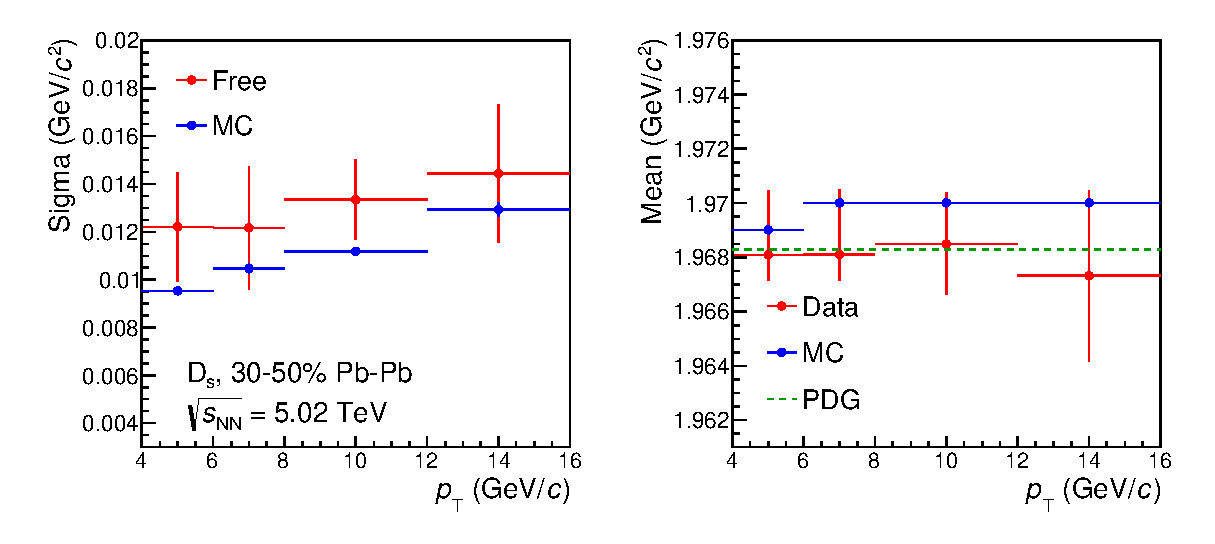
\includegraphics[width=15cm]{./FigCap5/DsMeanSigma_DataMC_3050.eps}
  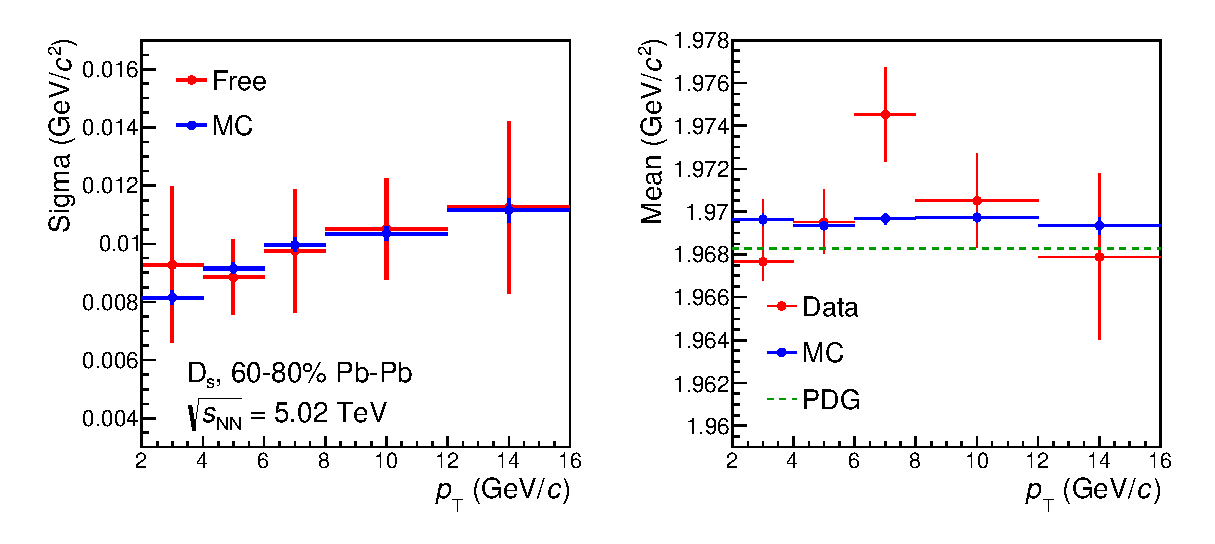
\includegraphics[width=15cm]{./FigCap5/DsMeanSigma_DataMC_6080.eps}
 \end{center}
 \caption{Gaussian width (left) and mean (right) of the $\Ds$ signal peak and as a function of $\pt$: values in data (red) are compared to values in MC (blue). For the mean of the peak, also the PDG value (green) is shown. }
 \label{fig:MCsigmacheckDs} 
\end{figure} 


 \begin{table}[!h]
 \begin{center}
  \begin{tabular}{|c|c|c|c|c|c|c|}
\hline
\multirow{2}{*}{$\pt$ bin (GeV$/c$)}& \multicolumn{2}{c|}{0-10$\%$} & \multicolumn{2}{c|}{30-50$\%$} & \multicolumn{2}{c|}{60-80$\%$} \\
\cline{2-7}
& raw yield & S/B & raw yield & S/B & raw yield & S/B \\
\hline
\hline
[2,4] & -  & - & -  & - & 42 $\pm$ 12 & 0.47 \\
\hline
[4,6] &  175 $\pm$ 32  & 0.20 & 141 $\pm$ 26  & 0.35 & 113 $\pm$ 17 & 0.63\\
\hline
[6,8] &  195 $\pm$ 36  & 0.16 & 162 $\pm$ 30 & 0.28 & 33 $\pm$ 7 & 3.08 \\
\hline
[8,12] & 137 $\pm$ 28 & 0.23 & 137 $\pm$ 18 & 0.86 & 40 $\pm$ 7 & 2.95 \\
\hline
[12,16] & 40 $\pm$ 8  & 1.90 & 56 $\pm$ 11 & 1.57 & 16 $\pm$ 5 & 2.10 \\
\hline
  \end{tabular}
 \caption{$\Ds$ raw yields and signal over background per $\pt$ interval for the three analysed centrality classes.}
  \label{tab:signalDs_010_3050_6080}
\end{center}
\end{table} 

\subsection{Corrections}
\label{sec:CorrectionsAA}
The $\Dspm$-meson raw yields were corrected in order to obtain the
$\pt$-differential yields of prompt $\Dsplus$ mesons: 
\begin{equation}
  \label{eq:dNdpt}
  \left.\frac{{\rm d} N^{\Dsplus}}{{\rm d}\pt}\right|_{|y|<0.5}=
  \frac{\left.f_{\rm prompt}(\pt)\cdot \frac{1}{2} N_{\rm raw}^{\rm
        \Dspm}(\pt)\right|_{|y|<y_{\rm fid}}}{\Delta\pt \cdot
    \alpha_y \cdot ({\rm Acc}\times\epsilon)_{\rm prompt}(\pt)
    \cdot{\rm BR} \cdot N_{\rm events}}\,.
\end{equation}
The raw yields $N_{\rm raw}^{\rm \Dspm}$ were divided by 
a factor of two to obtain the charge-averaged (particle and antiparticle) 
yields. To correct for the contribution of feed-down from B-meson decays,
 the raw yields were multiplied by the fraction of promptly produced D 
 mesons, $f_{\rm prompt}$. Furthermore, they were divided by the product 
 of prompt D-meson acceptance and efficiency 
 $({\rm Acc}\times\epsilon)_{\rm prompt}$, by the branching ratio {\rm BR} 
 of the decay channel, by the transverse momentum interval width 
 ($\Delta \pt$) and by the number of events ($N_{\rm events}$). The factor 
 $\alpha_y=y_{\rm fid}/0.5$ normalises the corrected yields measured in 
 $|y|<y_{\rm fid}$ to one unit of rapidity $|y|<0.5$, assuming a uniform 
 rapidity distribution for D mesons in the measured range. This assumption
  was validated to the 1\% level with simulations~\cite{ALICE:2011aa, Skands:2009zm}.

The correction for acceptance and efficiency $({\rm Acc}\times\epsilon)_{\rm prompt}$ 
was determined using Monte Carlo simulations with a detailed description 
of the detector and its response, based on the GEANT3 transport 
package~\cite{Brun:1994aa}. 
The underlying Pb--Pb events at $\sqrtsNN = 5.02$~TeV were simulated 
using the HIJING v1.383 generator~\cite{Wang:1991hta} and D-meson 
signals were added with the PYTHIA v6.421 generator~\cite{Sjostrand:2006za} 
with Perugia-2011 tune. Each simulated PYTHIA pp event contained a 
$\rm c\overline c$ or $\rm b\overline b$ pair, and D mesons were forced to 
decay into the hadronic channels of interest for the analysis. 
\begin{figure}[!b]
\includegraphics[width=.49\textwidth]{FigCap5/AccEff_Ds_010.pdf}
\includegraphics[width=.49\textwidth]{FigCap5/AccEff_Ds_3050.pdf}
\includegraphics[width=.49\textwidth]{FigCap5/AccEff_Ds_6080.pdf}
\caption{Efficiency times acceptance for $\Ds$ mesons in the three centrality classes, as a function of $\pt$, for prompt (red) and feed-down (blue) components.}
\label{fig:DsAccEff}
\end{figure}
The number of pp events added to each Pb-Pb 
event was adjusted according to the Pb-Pb collision centrality. 
The efficiencies were evaluated in a centrality class 
corresponding to the one used in 
data in terms of charged particle 
multiplicity, hence of the detector occupancy.
In the most central event class, the $\pt$ distribution 
of $\Ds$ mesons was weighted in order to match the 
shape measured for \mbox{$\rm D^0$ mesons} in finer 
$\pt$ intervals. In the other two centrality classes, 
where an analysis in finer $\pt$ intervals was not possible, 
the simulated $\Ds$-meson $\pt$ distribution was weighted 
to match the shape given by fixed-order next-to-leading-log 
perturbative QCD calculations (FONLL)~\cite{Cacciari:1998it,Cacciari:2001td} 
multiplied by the $\RAA(\pt)$ of D mesons computed 
using the BAMPS model for semi-central 
collisions~\cite{Uphoff:2011ad,Fochler:2011en,Uphoff:2012gb}.
Fig.~\ref{fig:DsAccEff} shows the acceptance-times-efficiency 
corrections for prompt and feed-down $\Ds$ mesons in the three
centrality classes.
Some of the topological selections tend to reject 
less feed-down due to the larger 
decay length with respect to the prompt D mesons. 
Other topological cuts, like the one on the normalised 
track-impact parameter residual, are more effective
in rejecting the feed-down component, allowing higher 
prompt efficiencies at high $\pt$.

{\bf Studies on the impact parameter resolution on the 
2015 data sample, revealed that this resolution is 
slightly worse (by about 5-10 micron at all $\pt$) 
than in Run-1 (e.g. 2011 Pb-Pb data).
The impact parameter distribution is shifted to negative 
values by up to 20-30 micron at low $\pt$ and 
decreasing to 5-10 micron at high $\pt$. The shift 
depends on the azimuthal angle and is not described 
in the MC. Current hypothesis is that part of the shift 
is due to the presence of SPD modules that were not 
included in the latest realignment (because they were
 included only recently in the data taking). The task 
 scales in the MC the residuals d0(true)-d0(reco) 
 according to the ratio data/MC of the impact parameter resolutions.}\\
 


The $f_{\rm prompt}$ factor was obtained, following the procedure 
introduced in~\ref{sec:BfdSub}, by subtracting the contribution of 
D mesons from B-meson decays from the measured raw yield 
in each $\pt$ interval. The expression for $f_{\rm prompt}$ reads:
\begin{equation}
\label{eq:fprAA}
\begin{split}
f_{\mathrm{prompt}} = \, & 1- \frac{N^{\text{D~feed-down}}_{\mathrm{raw}}}{N^{\mathrm{D}}_{\mathrm{raw}}}=\\
& 1- \RAA ^{\rm feed-down} \cdot  \langle \TAA \rangle \left (\frac{\rm d^2 \sigma}{\mathrm d\pt \mathrm d y} \right)^{\rm FONLL}_{\text{feed-down}} \cdot  \frac{(\mathrm{Acc} \times \epsilon)_\text{feed-down} \cdot \Delta y \Delta \pt \cdot \mathrm{BR} \cdot L_{\rm int}}{N^{\rm D +\overline{D},raw}/2}\,.
\end{split}
\end{equation}
The difference with respect to Eq.~\ref{eq:fpr} is that the beauty-hadron 
production cross section from FONLL pQCD
calculations for pp collisions at $\sqrt{s}=5.02~\tev$~\cite{Cacciari:2012ny}
is multiplied by $\langle \TAA \rangle$ of the corresponding centrality class. 
In addition, a hypothesis on the nuclear 
modification factor of feed-down $\Ds$ mesons, $\RAA^{\textnormal{feed-down}}$, was 
introduced to account for the different modification of beauty and charm 
production in Pb-Pb collisions. The resulting sample of 
feed-down $\Ds$ mesons is composed of two 
contributions: about 50\% of the feed-down originates from 
B$^0_{\rm s}$-meson decays, while the remaining 50\% comes from decays of 
non-strange B mesons (B$^0$ and B$^+$) (see Fig.~\ref{fig:DsParents}).
To determine the central value of $f_{\rm prompt}$ in the 0-10\% 
and 30-50\% centrality classes, it was assumed that the 
nuclear modification factors of feed-down and prompt $\Ds$ mesons were equal 
($\RAA^{\textnormal{feed-down}}=\RAA^{\rm prompt}$). 
The resulting feed-down contribution is about 10\%, depending on the
$\pt$ interval.
To determine the systematic uncertainty the hypothesis
was varied in the range $1/3<\RAA^{\textnormal{feed-down}}/\RAA^{\rm prompt}<3$, as 
discussed in detail in Section~\ref{sec:systematics}.
It should be noted that the central value and the range of the hypothesis
on $\RAA^{\textnormal{feed-down}}/\RAA^{\rm prompt}$ differ from those used for
non-strange D mesons in Refs.~\cite{ALICE-PUBLIC-2017-003,Adam:2015sza}. The 
central hypothesis of $\RAA^{\textnormal{feed-down}}/\RAA^{\rm prompt}$ for non-strange
D mesons is in fact set at 2  due to the comparison of the $\RAA$ of prompt D mesons at 
$\sNN = 2.76$ TeV~\cite{Adam:2015nna} with that of J/$\psi$ from B-meson decays~\cite{Khachatryan:2016ypw} 
measured in the CMS experiment (see Sec.~\ref{sec:resAAcap2}), that indicates that charmed hadrons 
are more suppressed than beauty hadrons. The hypothesis for $\Ds$ meson
accounts for the unknown role of 
recombination in the beauty sector, which
could enhance the ratio of B$^0_{\rm s}$ over non-strange B mesons~\cite{TAMULHC}, 
and for the large fraction of feed-down $\Ds$ mesons originating from non-strange B-meson decays.
For the peripheral class 60--80\%, in which the medium effects are milder, 
also the difference between charm and beauty mesons is assumed to be 
reduced: the value $\RAA^{\textnormal{feed-down}}=1.3\cdot\RAA^{\rm prompt}$ 
was used for all D-meson species. 


\section{Systematic uncertainty on corrected d$N$/d$\pt$}
\label{sec:systematics}
Most of the sources of systematic errors considered for the analysis 
of the corrected yield were already described in Sec.~\ref{sec:systPP}. 
Hence we will concentrate on the differences with respect to what 
already discussed. Table~\ref{tab:sysunc_yieldtable} summarises the 
assigned systematic uncertainties, as an example for the 0-10\% class. 

\subsection{Yield extraction systematics}
\label{sec:YieldExsystAA}
Since the two approaches described in 
Sec.~\ref{sec:RawYieldSyst} for the estimate of this 
systematic uncertainty were observed to give similar results,
for brevity the first approach is presented here. Fig.~\ref{fig:multitrial_Ds_010}
shows an example of the multiple trial fit procedure on the invariant-mass
distribution in the interval $4 < \pt < 6 \, \Gevc$, for the 0-10\% centrality class.
The panels of the figure show, starting from top left plot:
(i) the raw yield distributions from multiple trial extractions, 
with fit procedure and bin counting method 
in different colours; (ii) the distribution of raw yields from multiple 
trials, with the Gaussian width of the signal function as free parameter 
in the fit, fixed to its MC value or fixed to MC value $\pm$ 15\%; 
(iii) the reduced $\chi^{2}$ distribution of the fits; 
(iv) the Gaussian width of the peak as a function of the 
number of trials; (v) the raw yield distribution as a 
function of the number of trial; (vi) the RMS value (used as
estimator of the systematic uncertainty) of the yield distribution
in three cases: considering the fits with 
all possible values for the Gaussian sigma parameter (free, fixed to MC, fixed to MC $\pm$ 15\%), 
considering the fits with sigma free, fixed to MC, fixed to 
MC +15\% or finally with sigma free, fixed to MC, fixed to MC -15\%. 
In this way, for those $\pt$ intervals where the values 
of the sigma as free parameter were on average displaced towards 
values around MC sigma values +(-)15\%, the RMS of the second (third) 
distribution was chosen to give the final systematics. 
It was verified that the difference between the mean values of the yield distributions from fit
and from bin counting method was contained within the number quoted 
as systematic uncertainty.
The final assigned values range from 5\% to 10\% depending on $\pt$ and
centrality class. 



\begin{figure}[!htb]
 \begin{center}
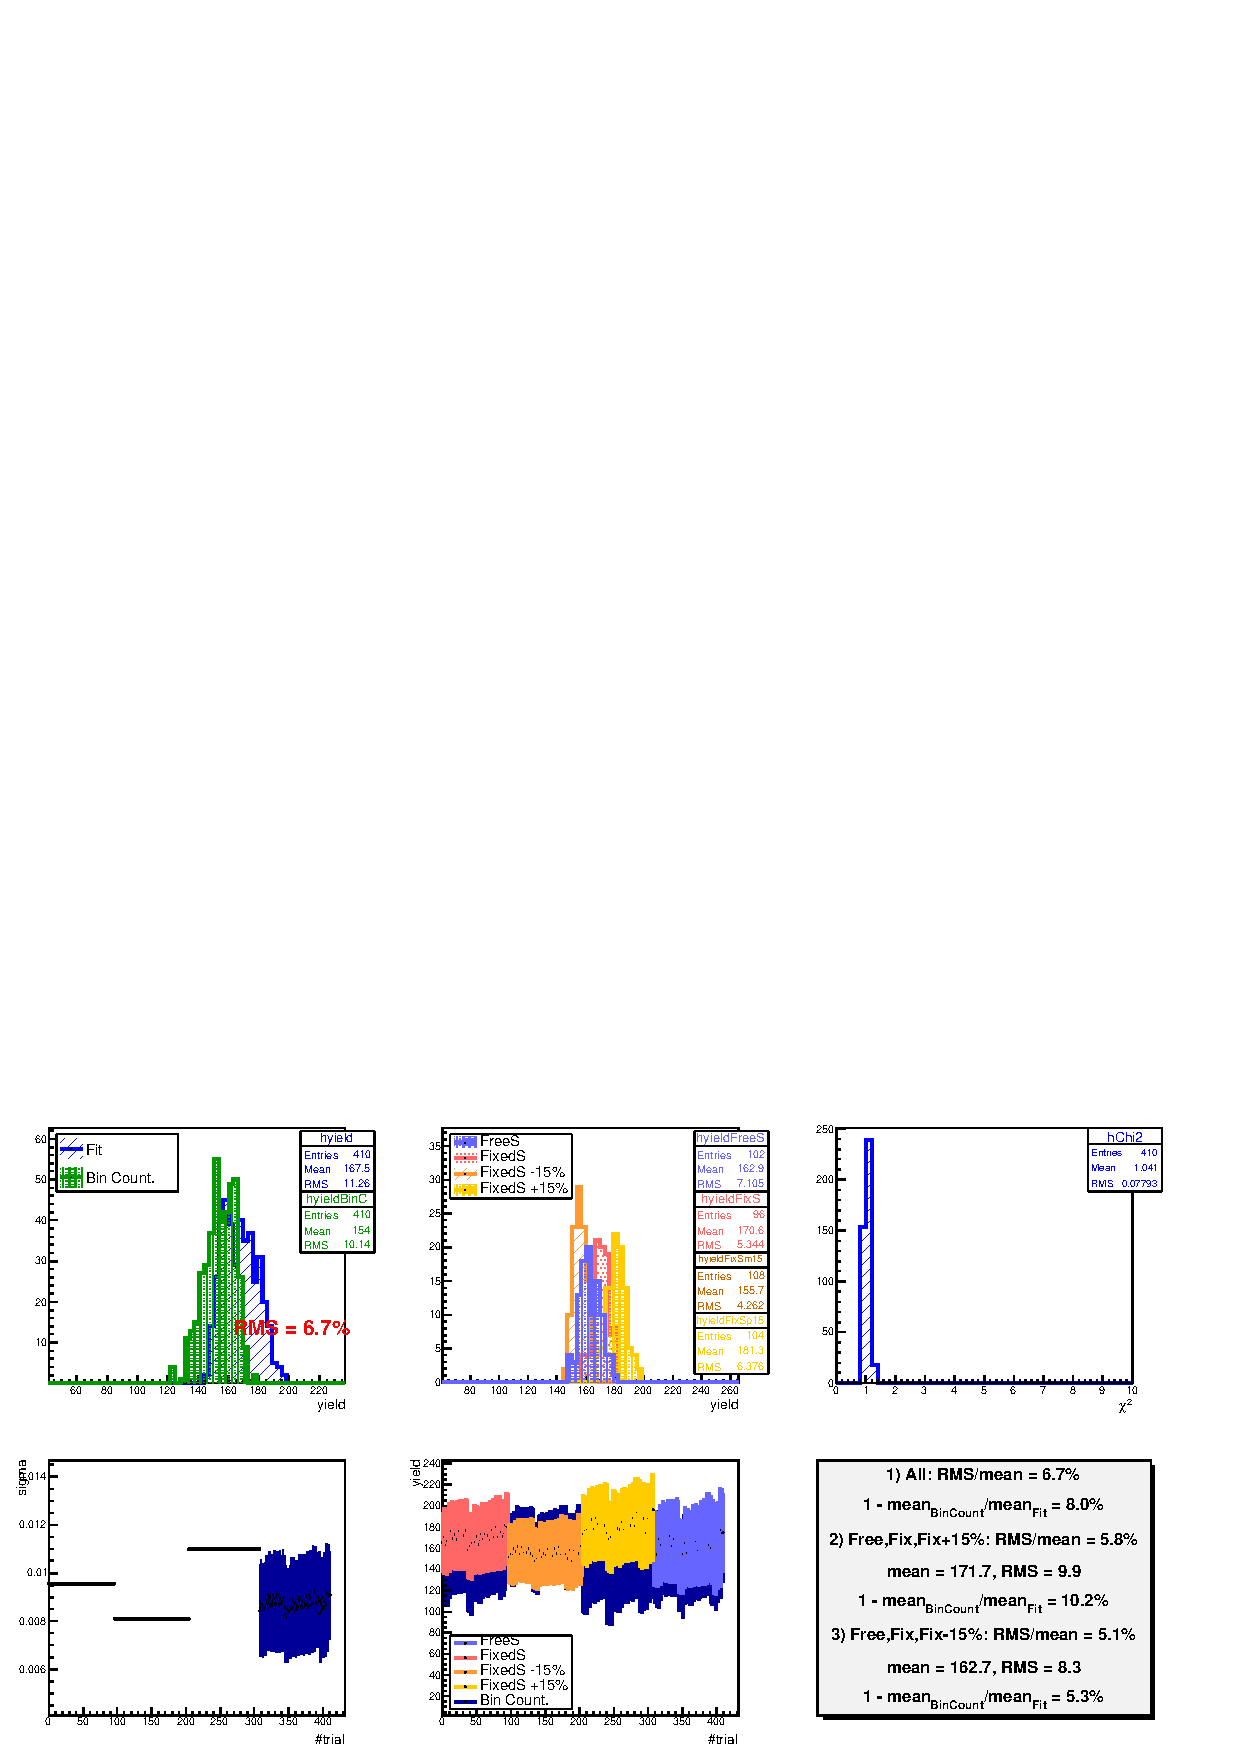
\includegraphics[width=15.cm]{./FigCap5/MT_Pt46_010.png}
\end{center}
 \caption{Output of multi-trial fits to $\Ds$ invariant mass distributions in the $\pt$ intervals 4-6 $\Gevc$  for the 0-10$\%$ centrality class.}
 \label{fig:multitrial_Ds_010}
\end{figure}


\begin{figure}[!h]
 \begin{center}
   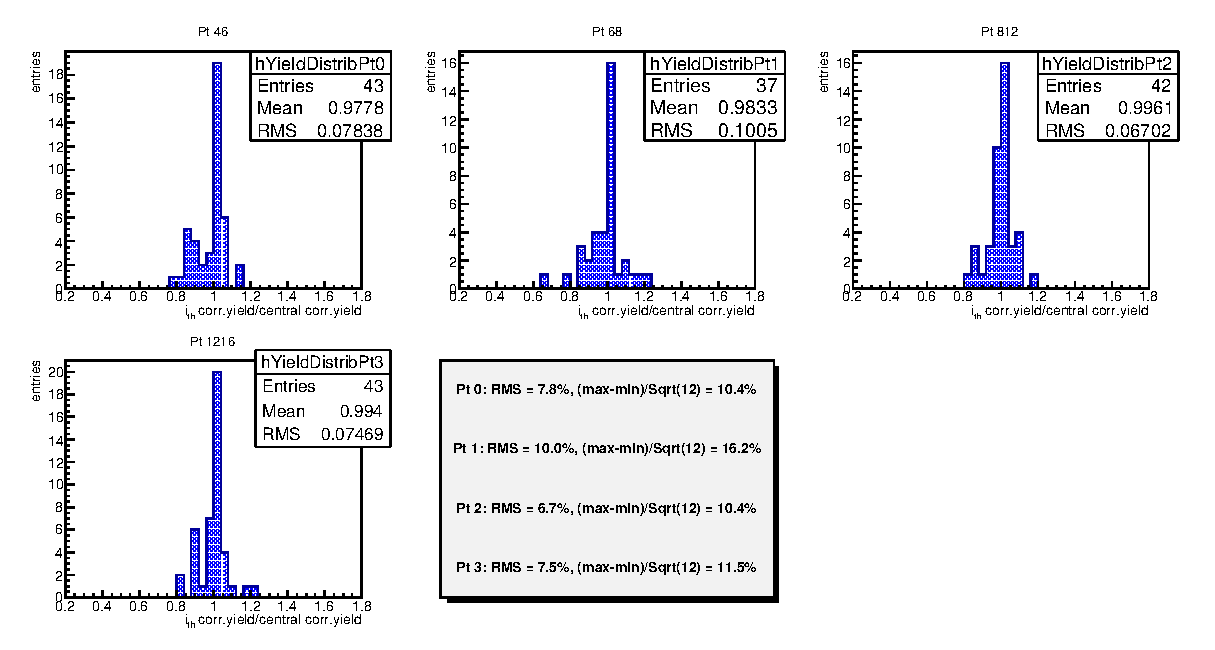
\includegraphics[angle=0, width=15cm]{./FigCap5/FinalSyst_010.eps}
 \end{center}
 \caption{Distribution of $\Ds$ corrected yields in the 0-10\% centrality class, obtained varying the selection on the topological variables with respect to the default value.}
 \label{DsCutVar_010} 
\end{figure}

\subsection{Topological selection efficiency}
\label{sec:CutVarsystAA}
A systematic scan from looser to tighter cuts was done on a variable-per-variable 
basis, reconstructing the yields, comparing them to the yields obtained 
with a reference set of cuts and looking for possible trends/biases of 
the reconstructed yield as a function of the cut strength.
The study was done using as reference set of cuts the one used 
to provide the central values of the yields. A selection
on the basis of the $\chi^2/ndf$ ($<2$) of the fits and the statistical significance ($>3$)
of the signal was applied. For the corrected yields that passed the selections
and that revealed systematics trends, their ratios to the reference corrected
yield, in each $\pt$ interval, were collected
into final distributions, used to provide the RMS values 
for the systematic uncertainty estimate. 
Fig.~\ref{DsCutVar_010} shows an example of such final distributions 
for the 0-10\% centrality class, in the four analysed $\pt$ intervals. 
The values of the RMS of Gaussian-like distributions are reported, as well as
the values of the full spread of the distribution divided by $\sqrt{12}$.

\subsection{PID selection efficiency}
\label{sec:PIDsystAA}
To estimate the effect of PID efficiency on the corrected yields, 
two particle identification selections (a tighter one, discussed in Sec.~\ref{Sec:PID}, and a 
looser, in Sec.~\ref{sec:PIDsystPP}) were compared. Fig.~\ref{fig:DsPID010} 
shows, as an example for 0-10\% centrality class, the ratio of the corrected yields 
with looser and tighter PID selection. Due to the large error bars, it is difficult to asses
whether the points are affected by a (considerable, $\sim$15-20\%) systematic effect
or they are simply dominated by statistical fluctuations originating from
yield extraction. For this reason, an alternative approach of a per-track 
systematic was followed. The idea is to apply optimised selections in data to obtain
pure samples of kaons and pions. The difference in the efficiencies for a given N$\sigma$ cut (on d$E$/d$x$ or 
time-of-flight signal) in data and MC will
constitute a $\pt$-dependent per-track systematics for each species.
The per-track systematics can be propagated to the D-meson level, via the kinematics of
the tracks of the daughters.
\begin{figure}[!h]
 \centering
 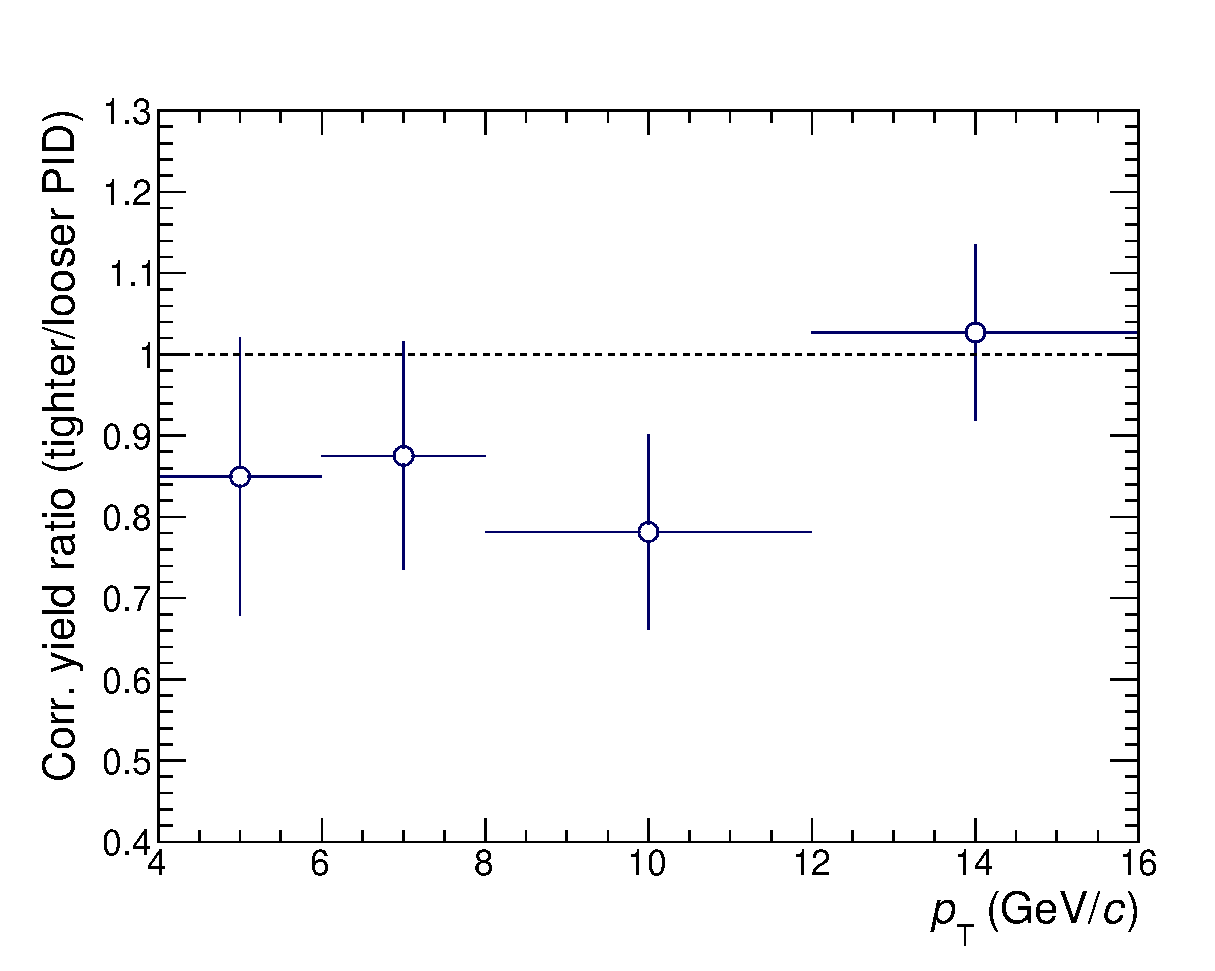
\includegraphics[angle=0, width=7cm]{./FigCap5/PIDsyst_010.eps}
 \caption{Ratio of $\Ds$ corrected yield in 0--10\% centrality class with tighter-to-looser PID selections.}
 \label{fig:DsPID010} 
\end{figure}
Pions from V0 decays were selected using the optimised cuts
used in~\cite{Schuchmann:2102194}. In Fig.~\ref{fig:MCPionsTPC} the Monte Carlo 
N$\sigma$ distributions for the d$E$/d$x$ of pions in TPC are shown for 
different $\pt$ intervals, from 0.2 to 10 $\Gevc$.
The N$\sigma$ distribution of true pions (in green) is compared to the
distribution of tracks in the simulation that pass the selection as pions from V0 decays 
(in blue). Since a second population is visible on the right of the 
peak at low $\pt$ for
the blue distribution (as well as in data, likely a contamination from electrons), 
only the left region of the peak will be used 
to evaluate the efficiency of the N$\sigma$ cuts.
A part from this secondary population, in general the comparison is good and we
conclude that the utilised selections provide a good
cleaning of the sample. 
In Fig.~\ref{fig:DataPionsTPC}, the N$\sigma$ distributions in data (blue) are compared
to the distributions of true MC pions (green), in the different $\pt$ intervals.  
Finally, efficiencies in data and in MC are obtained by integrating the respective 
distributions (blue and green distributions in Fig.~\ref{fig:DataPionsTPC})
within 1, 2 or 3$\sigma$, and normalising these values to the integral 
of the distributions within 5$\sigma$. It was verified that enlarging the number of $\sigma$ from 5 to 10 at the 
denominator of the efficiency does not affect the final results.
The same procedure
was carried out with distributions of time-of-flight signals in TOF
for the above selected pions, to obtained the systematics on pion identification in TOF.
To obtain the uncertainty on kaon identification in TPC, a tight cut on the PID 
signal in TOF requiring N$\sigma < 0.25\sigma$ from kaon hypothesis was required. 
The black curve in Fig.~\ref{fig:MCKaonsTPC}, for PID signal in TPC, was obtained
from reconstructed track in the simulation that satisfy this selection.
Contaminations from other particle species are still present and they
are shown in different colours in the same Fig.~\ref{fig:MCKaonsTPC}. 
The black curve was fitted with a Gaussian shape 
to extrapolate the kaon contribution. The ranges of the fits are set, for each $\pt$ interval, in 
the regions less affected by other species contribution.
In Fig.~\ref{fig:DataKaonsTPC}, the distribution of d$E$/d$x$ in data is displayed. 
The yellow Monte Carlo template of true 
kaons is superimposed to the data distribution, 
only for visualisation purposes, and not used in the fit. The curve in data
was fitted with a Gaussian function in the $x$-axis range previously tuned with the MC,
to extrapolate the kaon component from the inclusive distribution, in each $\pt$ interval.\\
The values of the final systematics, obtained as the data-to-MC ratio
of the efficiencies are shown in Fig~\ref{fig:PerTrackPIDsys}, as a function of $\pt$,
for cuts at 1, 2 ans 3$\sigma$ on the PID signal. 
Since the systematic uncertainties on pion and kaon identification in 
TPC show similar values, an assumption for the systematic uncertainty 
on kaon identification in TOF is done and it is considered to be similar to that of pions in TOF.
These $\pt$-dependent per-track values were then associated to
$\Ds$' daughter tracks, depending on their transverse momentum, and linearly summed together 
for each candidate. The topological discussed 
in Sec.~\ref{sec:CutVarsystAA} were applied. 
The final values of the systematic uncertainties are around 
3\% for the tighter PID selection (Sec.~\ref{Sec:PID}) and are negligible for the
looser PID selection (Sec.~\ref{sec:PIDsystPP}).

\begin{figure}[!h]
 \centering
 \includegraphics[angle=0, width=15cm]{./FigCap5/PionTPC_MC.png}
 \caption{N-sigma distribution for dE/dx signal in TPC from pion hypothesis in Monte Carlo. In green pions selected by PDG code, in blue and in red pions passing the selection for V0 decays without and with PDG code selection respectively.}
 \label{fig:MCPionsTPC} 
\end{figure}

\begin{figure}[!h]
 \centering
 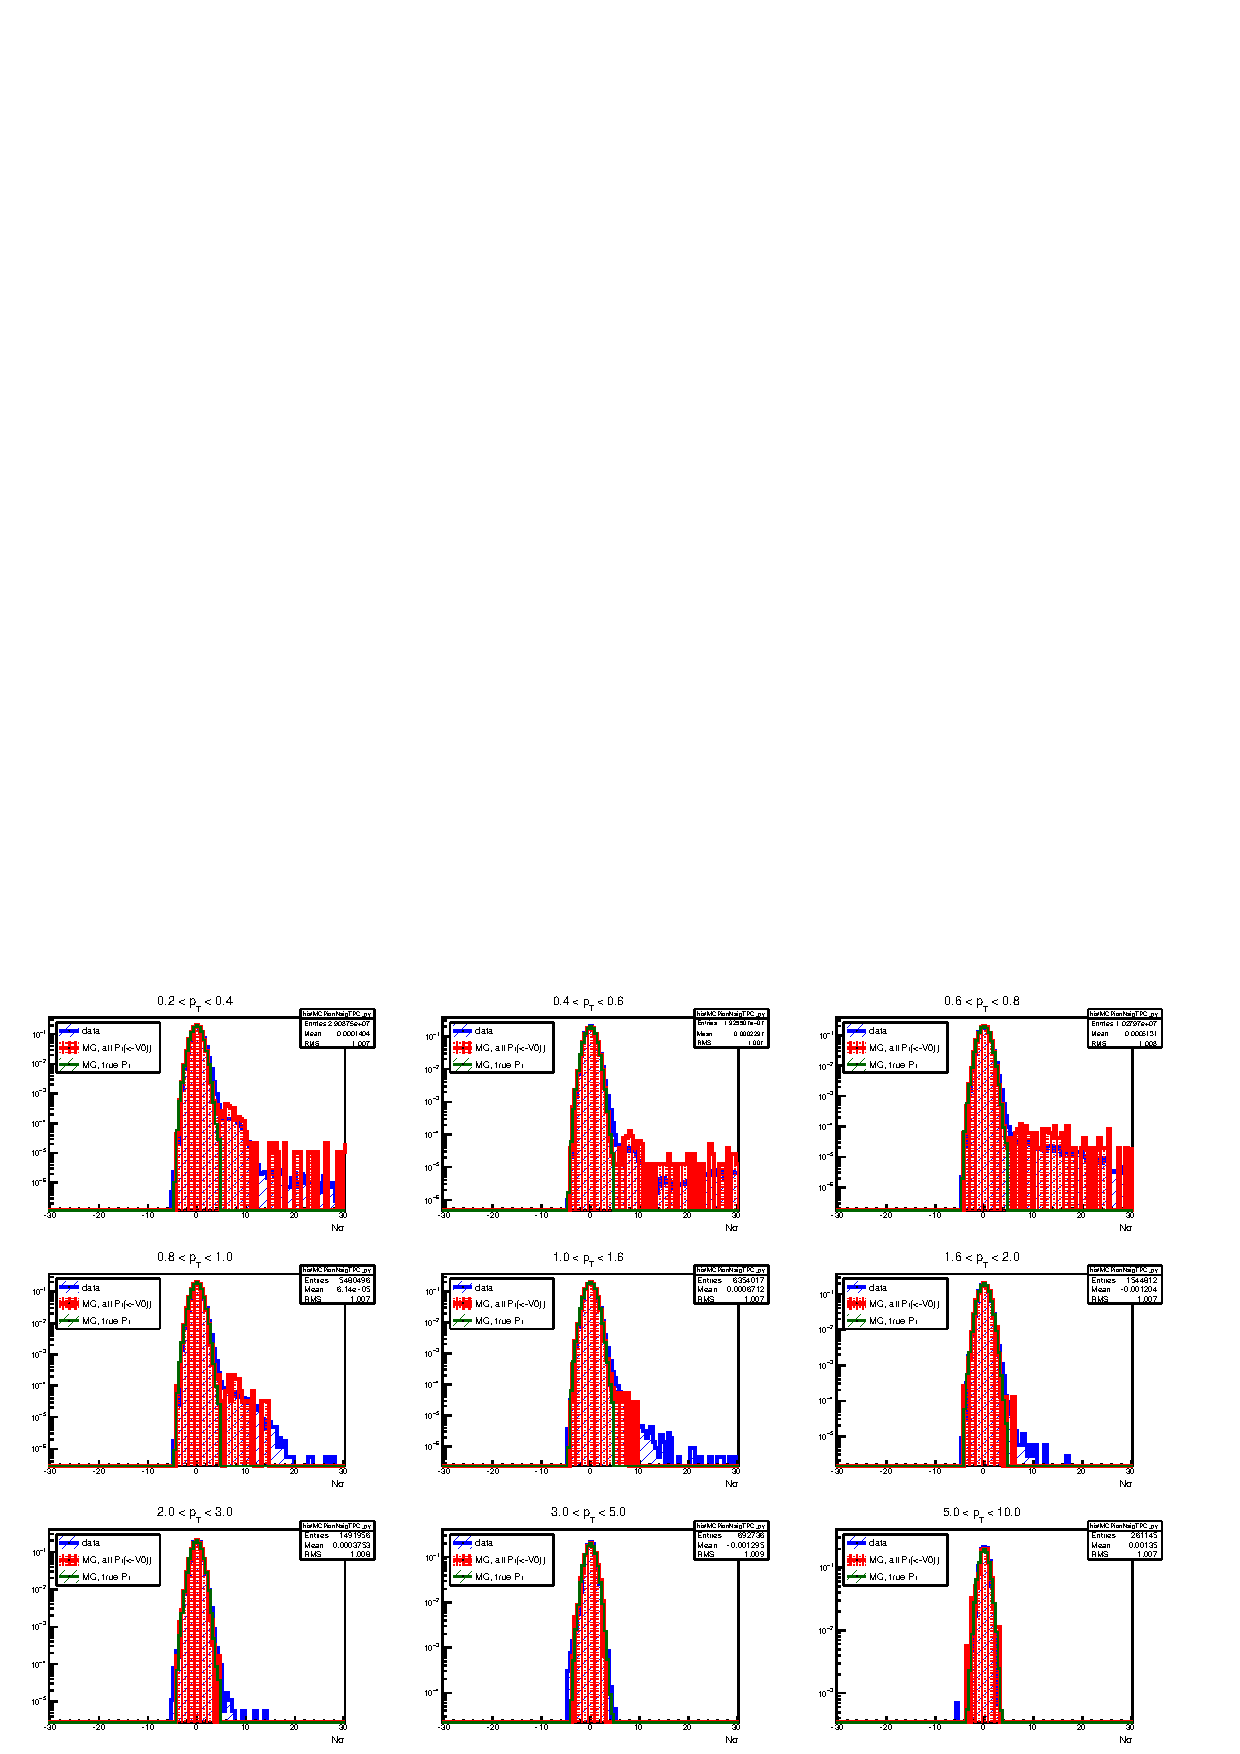
\includegraphics[angle=0, width=15cm]{./FigCap5/PionTPC_DataMC.png}
 \caption{N-sigma distribution for dE/dx signal in TPC from pion hypothesis in data and Monte Carlo. In green pions selected by PDG code, in blue and red pions passing the selection for V0 decays in Monte Carlo and data respectively.}
 \label{fig:DataPionsTPC} 
\end{figure}

\iffalse
\begin{figure}[!h]
 \centering
 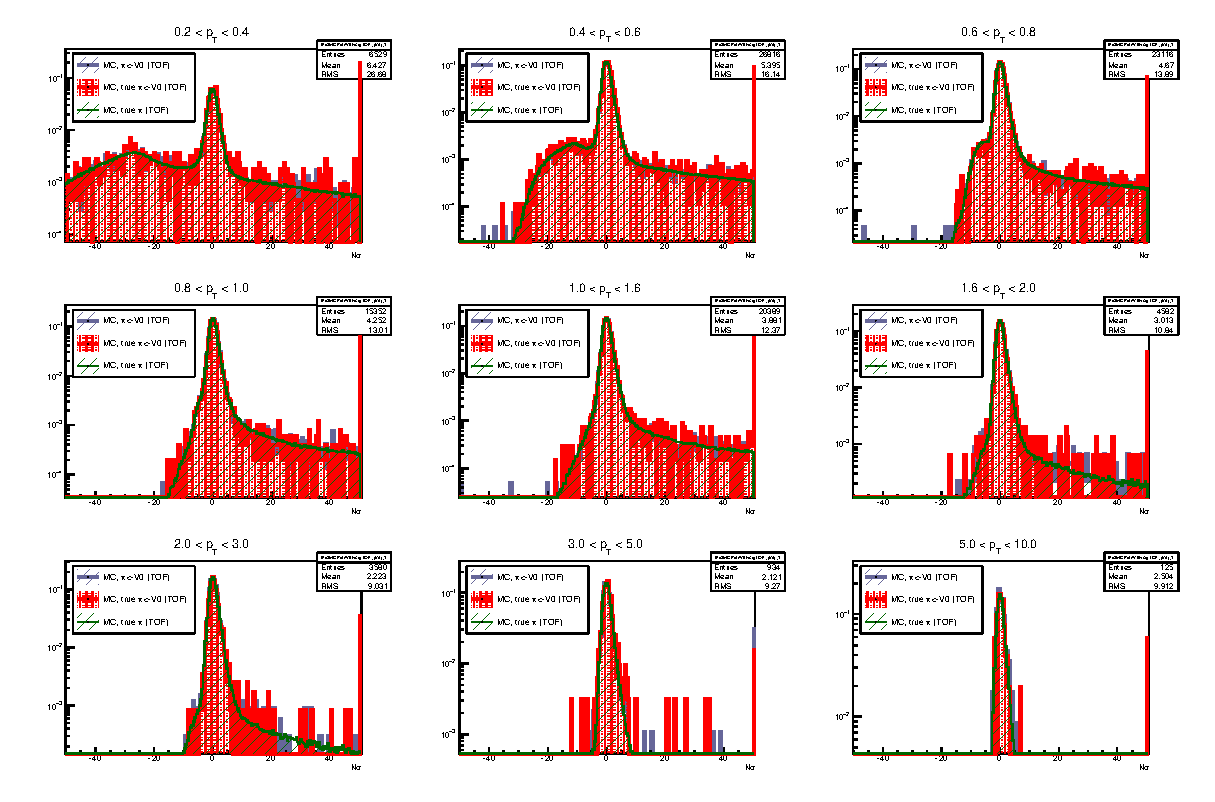
\includegraphics[angle=0, width=13cm]{./FigCap5/MCPionTOF_AllTrueSig.eps}
 \caption{N-sigma distribution for t.o.f. signal in TOF from pion hypothesis in Monte Carlo. In green pions selected by PDG code, in blue and in red pions passing the selection for V0 decays without and with PDG code selection respectively.}
 \label{fig:MCPionsTOF} 
\end{figure}
\fi

\begin{figure}[!h]
 \centering
 \includegraphics[angle=0, width=15cm]{./FigCap5/KaonTPCFromTOF_MC.png}
 \caption{N-sigma distribution for dE/dx signal in TPC from kaon hypothesis in Monte Carlo, after a cut at sigma $<$ 0.25 from kaon hypothesis for TOF signal. In yellow, contribution from true kaons, in magenta from pions and in green from protons. In red, the fit to extrapolate the kaon component in the inclusive distribution.}
 \label{fig:MCKaonsTPC} 
\end{figure}

\begin{figure}[!h]
 \centering
 \includegraphics[angle=0, width=15cm]{./FigCap5/KaonTPCFromTOF_DataMC.png}
 \caption{N-sigma distribution for dE/dx signal in TPC from kaon hypothesis in data, after a cut at sigma $<$ 0.25 from kaon hypothesis for TOF signal. In yellow, contribution from true kaon superimposed to data. In red, the fit to extrapolate the kaon component in the inclusive distribution.}
 \label{fig:DataKaonsTPC} 
\end{figure}

\begin{figure}[!h]
 \centering
 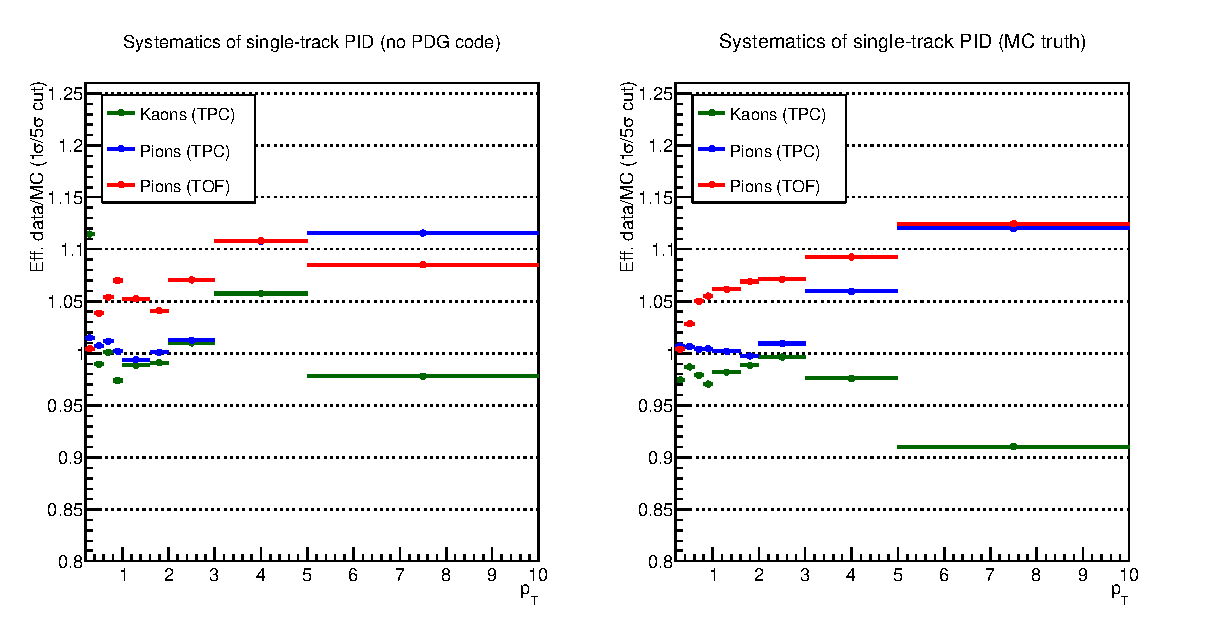
\includegraphics[angle=0, width=7cm]{./FigCap5/PIDsyst_1over5sigmaCut.eps}
 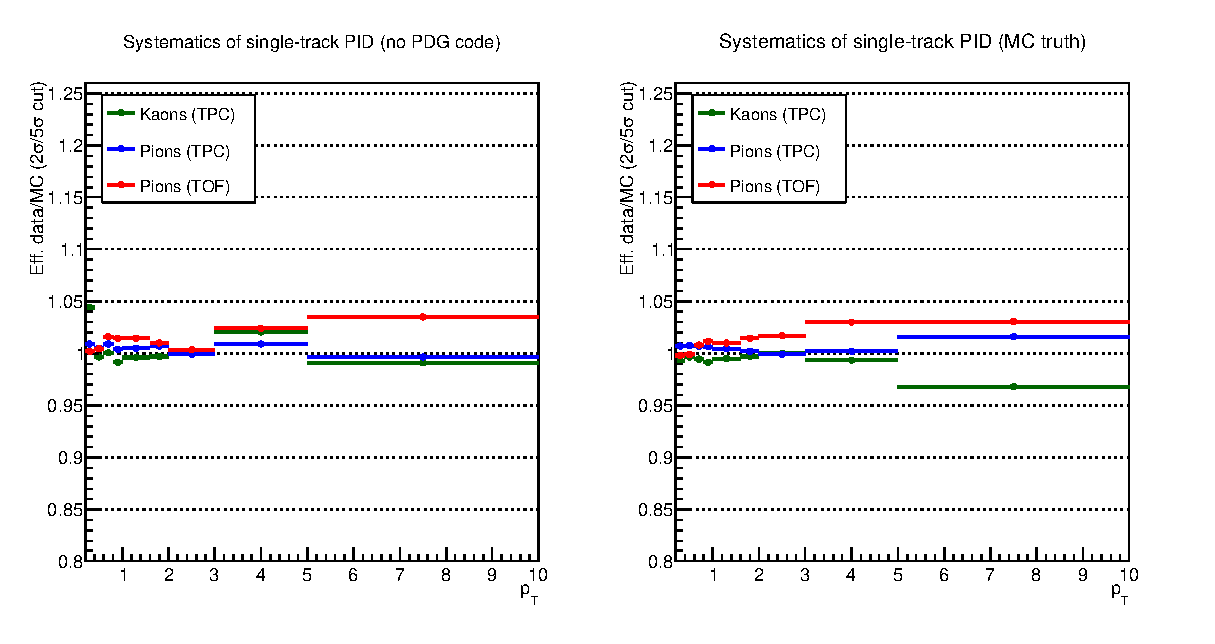
\includegraphics[angle=0, width=7cm]{./FigCap5/PIDsyst_2over5sigmaCut.eps}
 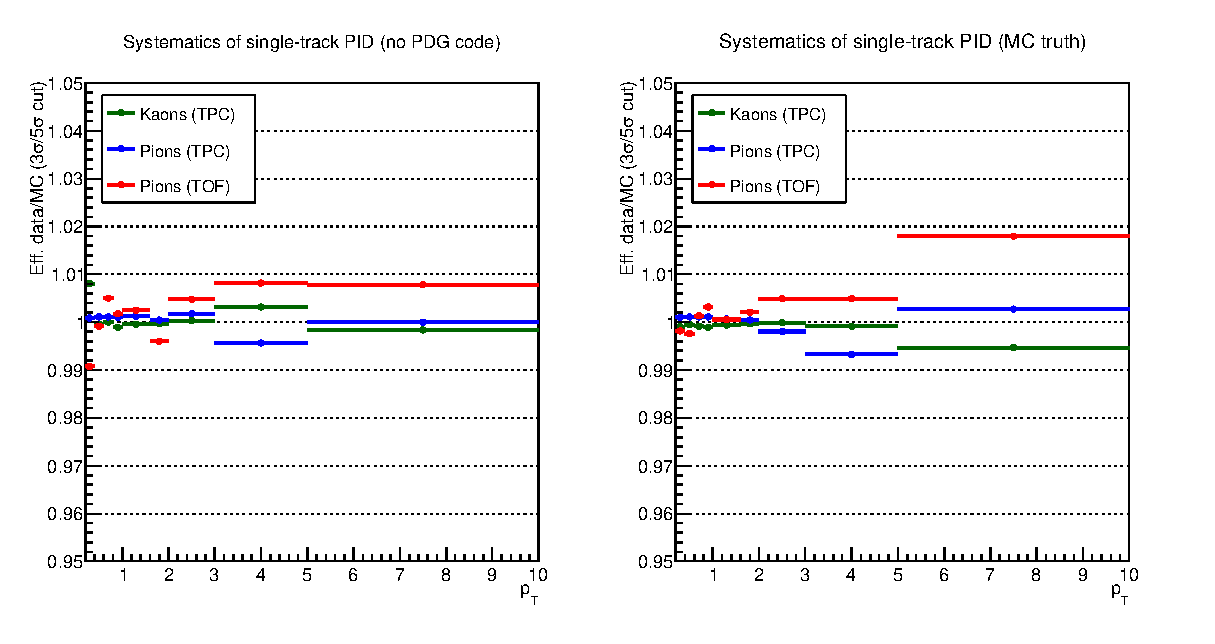
\includegraphics[angle=0, width=7cm]{./FigCap5/PIDsyst_3over5sigmaCut.eps}
 \caption{Per-track systematics for kaons and pions in TPC and TOF in different colours, as a function of $\pt$, for 1, 2 and 3$\sigma$ selection, normalised to a 5$\sigma$ cut. }
 \label{fig:PerTrackPIDsys} 
\end{figure}

\begin{figure}[!h]
 \centering
 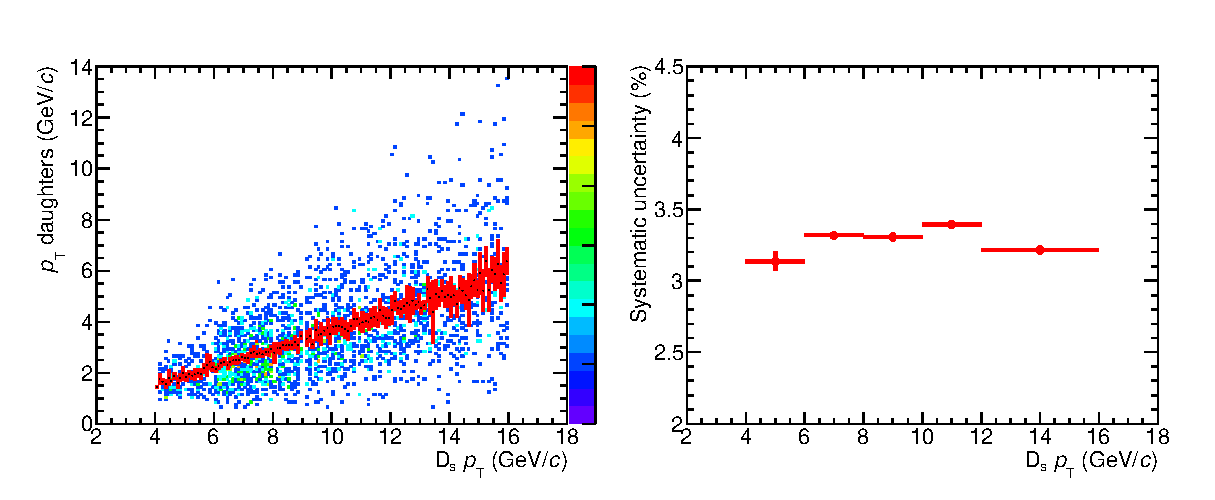
\includegraphics[angle=0, width=13cm]{./FigCap5/PIDsystDs_MCall.eps}
 \caption{Left: scatter plot of $\Ds$ daughter $\pt$ as a function of $\Ds$ $\pt$. Right: systematics on the tighter PID selection used for $\Ds$ meson as a function of $\pt$.}
 \label{fig:DsPIDsys} 
\end{figure}

\subsection{Generated $\pt$ shape}
The systematic effect on the efficiency due to a possible difference between 
the real and simulated $\Ds$-meson transverse momentum distributions
was estimated by using alternative $\Ds$-meson $\pt$ distributions.
In particular, the $\pt$ distributions from FONLL calculations with
and without hot-medium effects parametrised based on the $\RAA$ in central collisions from the 
TAMU~\cite{He:2014cla} model and in semi-central collisions from 
BAMPS~\cite{Uphoff:2014hza} model were used in this study.
The values assigned as systematic uncertainty are reported in 
Table~\ref{tab:sysunc_yieldtable} for the 0-10\% centrality class, but are similar in 
30-50\% and 60-80\% classes. 

\iffalse
\begin{figure}[!htp]
\begin{center}
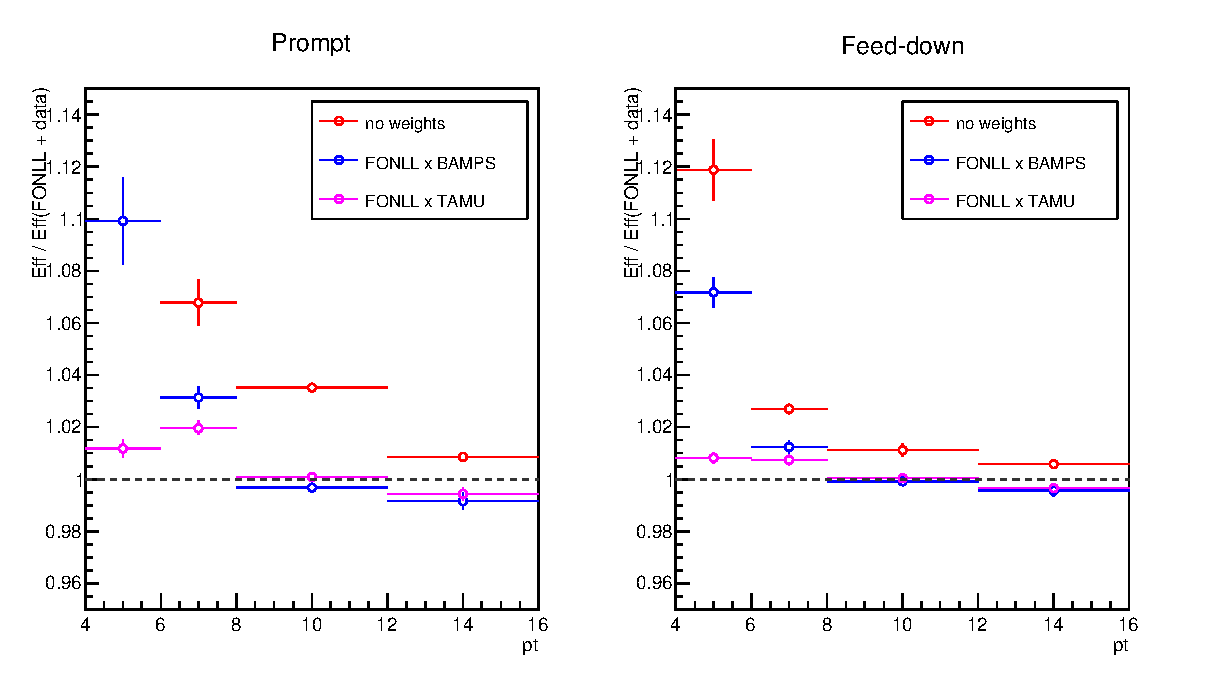
\includegraphics[angle=0, width=11.cm]{./FigCap5/MCptweights010_overFONLLdata_617.eps}   
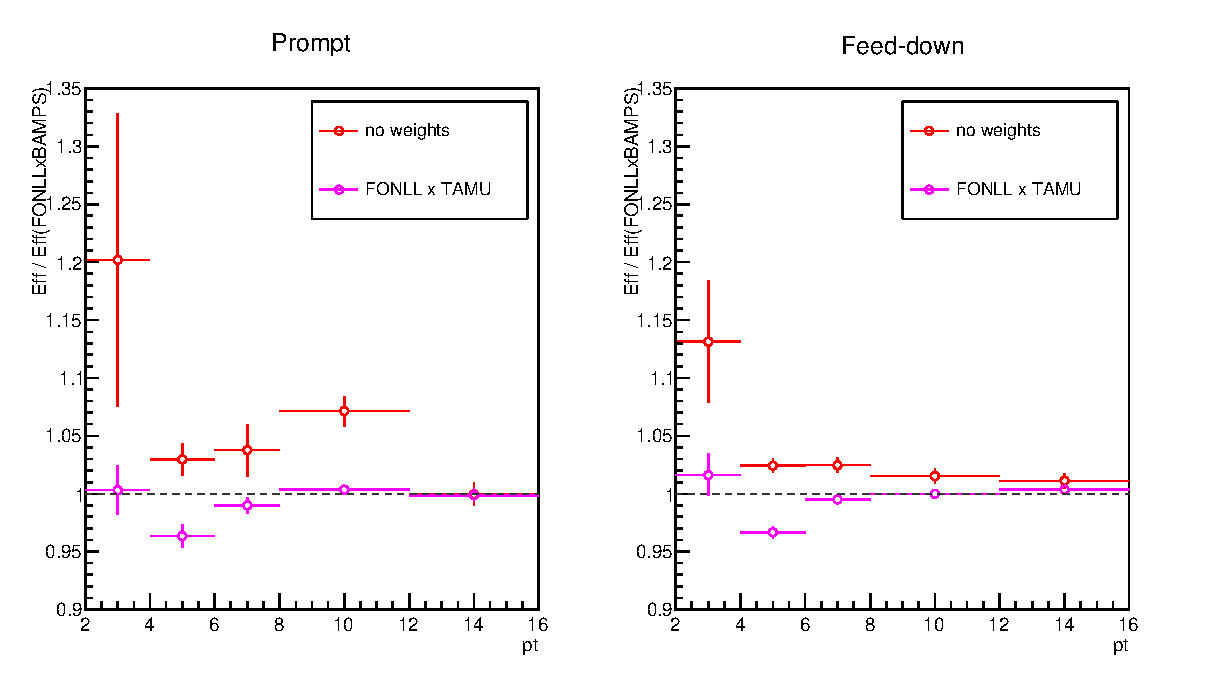
\includegraphics[angle=0, width=11.cm]{./FigCap5/MCptweights6080_overFONLLBAMPS_618.eps}   
\end{center}
\caption{Top: relative change of $\rm \Ds$ prompt and feed-down efficiencies in the 0--10\% centrality class by using FONLL  x BAMPS (blue), no (red) $\pt$-weights, or FONLL x TAMU (magenta) with respect to case of $\Dzero$ data-driven weights (default). Bottom: relative change of $\rm \Ds$ prompt and feed-down efficiencies in the 60--80\% centrality class by using no (red) $\pt$-weights, or FONLL x TAMU (magenta) with respect to case of FONLL x BAMPS weights (default).}
\label{DsMCshape_010_6080} 
\end{figure}
\fi

\subsection{Feed-down subtraction}
The systematic uncertainty on the subtraction of feed-down from 
B-meson decays was estimated by varying i)
the $\pt$-differential feed-down D-meson cross section from the 
FONLL calculation within the theoretical uncertainties (that originate from variations on 
$b$-quark mass, perturbative scales and on the parton distribution functions~\cite{Cacciari:2012ny}), 
ii) the ratio of the prompt and feed-down $\Ds$-meson $\Raa$ in the 
range $\frac{1}{3} < \RAA^{\rm  feed-down}/\RAA^{\rm prompt} < 3$ 
for the centrality classes 0-10\% and 30-50\%. The range was limited to 
$1 < \RAA^{\rm  feed-down} / \RAA^{\rm prompt} < 1.6$ 
for the centrality class 60-80\%. 

\subsection{Track reconstruction efficiency}
\label{sec:TrackEffSystPbPb}
The procedure to estimate the difference
of tracking efficiency between data and MC was discussed in Sec.~\ref{sec:TrackEffSystPP}.
The per-track uncertainty quoted to account for track-quality selection efficiencies
is 1.5\% in the 10\% most central events and 1\% in 30-50\% and 60-80\% 
centrality classes. As regards the systematic uncertainty from ITS-TPC track
matching efficiency, some discrepancies (up to 4\%, for $2 < \pt < 4\, \Gevc$) 
are observed in the final systematics for Pb-Pb data
when switching off the request of a hit in one of the two SPD 
layers for the tracks used to perform the DCA$_{\rm xy}$ fits.
As explained in Sec.~\ref{sec:TrackEffSystPP}, this request is 
preferable since the DCA$_{\rm xy}$
resolution is more accurate, thus differences between primary and secondary track DCA$_{\rm xy}$ 
distributions can be appreciated. This request also implies 
a correction factor to rescale the fraction of primary tracks in the ITS
to the same fraction in TPC. Such factor is extracted from MC and it
lays on the hypothesis that simulation can reproduce the ITS-to-TPC ratio of primary tracks 
as in data. For the case 
without the request of hit in the SPD, the DCA$_{\rm xy}$
resolution is worse, but the fits can be performed with still acceptable data-to-fit agreement.
The observed discrepancy in the results from the two cases 
may be due to the less precise estimate
of the fraction of primary tracks due to looser resolution power as well as
a non valid assumption for the correction factor. For this reason, the systematic 
uncertainty on the ITS-TPS matching efficiency was
assigned by averaging the two results, resulting in
2.5-4\% for $0.5 < \pt < 5 \, \Gevc$, 2.5-1\% for $5 < \pt < 10 \, \Gevc$, 1\% for $10 < \pt < 15\, \Gevc$.


\begin{table}[!h]
\centering
\begin{tabular}{|l|l|l|c|c|c|c|c|}
\hline
\multicolumn{6}{|c|}{0--10\% centrality class}       \\                                                                                                                                                                                                                                               \hline
$\pt$ interval ($\gev/c$)           & 2--4        &    4--6          & 6--8      &   8--12            & 12--16                  \\ 
Yield extraction & & & & & \\
Tracking efficiency & & & & & \\
PID efficiency & & & & & \\
Cut efficiency & & & & & \\
MC $\pt$ shape & & & & & \\
Feed-down subtraction & & & & & \\
Branching ratio & & & & & \\
Centrality limit & & & & & \\
Data syst. in pp and $\sqrt s$-scaling of the pp ref. & & & & & \\
\hline
\end{tabular}
\caption{Relative systematic uncertainties on the $\RAA$ of $\Ds$ in the 0-10\% centrality class.}
\label{tab:sysunc_yieldtable}
\end{table}

\section{Nuclear modification factor in Pb-Pb collisions}
\label{sec:RAA}
The nuclear modification factor $\RAA$ of prompt $\Dsplus$ mesons was defined as follows:
\begin{equation}
\label{eq:RAADs}
\RAA (\pt) = \frac{1}{\langle \TAA \rangle} \frac{{\rm d} N_{\rm AA}/{\rm d}\pt}{{\rm d} \sigma_{\rm pp}/{\rm d} \pt},
\end{equation}
where ${\rm d} N_{\rm AA}/{\rm d}\pt$ is the corrected $\pt$-spectrum of 
Eq.~\ref{eq:dNdpt}, $\langle \TAA \rangle$ is the 
average nuclear overlap function and ${\rm d} \sigma_{\rm pp}/{\rm d} \pt$ is 
proton-proton reference at $\s = 5.02$ TeV.
\section{Systematic uncertainty on the $\RAA$}
\label{sec:SystRAA}
The systematic uncertainties on the $\Raa$ measurement include those 
on the $\Ds$-meson corrected $\pt$-spectrum described above. The systematic 
uncertainty on the feed-down subtraction deriving from
the variation of the parameters of the FONLL calculation was considered to be
correlated in the $\PbPb$ and pp measurements. All the 
other sources of systematic uncertainties were treated as uncorrelated. 
Additional systematic uncertainties on the $\Raa$ are on 
the proton--proton reference cross section and on the $\RAA$ normalisation. 

\subsection{Proton-proton reference}
\label{sec:PPrefSyst}
The $\pt$-differential cross section of prompt $\Dsplus$ mesons with 
$|y|<0.5$ in pp collisions at $\sqrt s=5.02~\tev$, used as reference 
for the nuclear modification factor, was obtained by scaling the 
measurement at $\sqrt{s}=7~\TeV$ described in 
Chapter~\ref{chap:pp}~\cite{Acharya:2017jgo} to $\s = 5.02$ TeV 
with FONLL calculations~\cite{Cacciari:2012ny}. This measurement 
reaches up to $12~\Gevc$ for $\Ds$ mesons.
The uncertainty on the pp reference 
has two contributions. The first one is the global uncertainty on the measured 
$\pt$-differential $\Dsplus$-meson cross section at $\sqrt s=7$~TeV.
The second contribution is the $\pt$-dependent scaling factor 
from $\sqrts=7~\tev$ to $\sqrts=5.02~\tev$, determined by varying
the FONLL parameters (charm-quark mass, factorisation and renormalisation scales) 
as described in~\cite{Averbeck:2011ga}. This uncertainty ranges from 
$^{+17}_{-\phantom{1}4}\%$ for $1<\pt<2~\gev/c$ to about $\pm3\%$ for $\pt>10~\gev/c$.
In the interval $12<\pt<16~\Gevc$, the FONLL calculation at 
$\sqrt s=5.02~\tev$~\cite{Cacciari:2012ny} was used as a reference 
by scaling the values to match the central value of the data at lower $\pt$. 
This procedure is described in Ref.~\cite{Adam:2015sza}. The total 
systematic uncertainty on the $\pt$-extrapolated cross section is about 
$^{+42}_{-29}\%$ for $\Ds$ in the $\pt$ interval 12--16~$\Gevc$.


\subsection{Normalization}
\label{sec:NormalizSyst}
The uncertainties on the $\RAA$ normalisation are the quadratic sum of 
(i) the pp normalisation uncertainty (3.5\%), 
(ii) the uncertainty on $\langle T_{\rm AA} \rangle$, which ranges from 3.3\% to 6.2\% depending on the centrality, and
(iii) the uncertainty on the fraction of the hadronic cross section used in the 
Glauber fit to determine the centrality ($<0.1\%$, $2\%$ and $3\%$ for the 0--10\%, 30--50\% 
and 60--80\% centrality classes, respectively)~\cite{Adam:2015sza}, while the branching ratio uncertainty cancels out in the 
ratio.

\section{$\Ds$ elliptic flow}
In this section, the first measurement at LHC of the $v_2$ of 
$\Ds$ meson in Pb--Pb collisions at 
$\sqrtsNN = 5.02$~$\TeV$ is reported. The analysis was carried 
out for the 30-50\% centrality class, because it is the centrality
interval where the elliptic flow reaches its maximum value~\cite{Adam:2016izf}. 

\subsection{Event characterization: event plane}
\label{sec:EventPlane}
Let's briefly recall that the reaction plane ($\Psi_{\rm RP}$) is the 
plane formed by the impact parameter of the two colliding nuclei and the beam
direction. The orientation of the reaction plane or, in case of flow fluctuations, 
of the $n^{th}$-harmonic collision symmetry plane is estimated 
from the particle azimuthal distribution event-by-event
with the $n^{th}$-harmonic event-plane angle, $\psi_n^{\rm EP}$.
For a given harmonic $n$, one constructs the two-dimensional event-plane 
vector $\vec{Q}_n$ from the measured azimuthal distribution of 
particles produced in the event as follows:
\begin{equation}
\label{f:qvector}
 \vec{Q}_n= {Q_{n,x} \choose Q_{n,y}} = {\sum_{i=0}^{N} w_i \cos (n\varphi_i) \choose \sum_{i=0}^{N} w_i \sin (n\varphi_i)}.
\end{equation}
The sums run over all reconstructed tracks in the case 
of the TPC, or segments of detectors with azimuthal 
segmentation like V0 or ZDC. The angle $\varphi_i$ is 
the azimuthal emission angle of the $i^{th}$ particle or the 
azimuthal coordinate of the $i^{th}$ detector element, respectively. 
For TPC tracks the weight $w_i$ can be unity or a specific 
function of $\pt$, useful to enhance the 
contribution of particle with large flow, improving 
the resolution on the event plane. For segmented detectors, $w_i$ is the 
signal observed in the $i^{th}$ detector element. The observed plane 
angle of the $n^{th}$ harmonic is given by the orientation of $\vec{Q}_n$:
\begin{equation}
\psi_n = \dfrac{1}{n} \tan^{-1} \left(\dfrac{Q_{n,y}}{Q_{n,x}}\right).
\end{equation}
Due to the finite number of detected particles, the
angular resolution on reaction plane $\Psi_{\rm RP}$ is limited and 
has be estimated for the $n^{th}$ harmonic as:
\begin{equation}
R_n = \langle {\rm cos}[n({\rm \psi}_n-{\rm \Psi}_{\rm RP})]) \rangle ,
\end{equation}
where the angle brackets denote an average over a large event sample.
The resolution term must be used to correct the flow coefficients as:
\begin{equation}
v_n = \frac{v_n^{obs}}{R_n}.
\end{equation}
It can be demonstrated that the the event plane resolution 
can be expressed as:
\cite{Poskanzer:1998yz}:
\begin{equation}
\label{eq:epreso}
\left\langle \cos [km\left( \psi_m-\Psi_{\rm RP}\right)]\right\rangle = \sqrt{\dfrac{\pi }{8}} \chi_m \cdot {\rm e}^{-\chi_m^2/4} \cdot I_{(k-1)/2}(\chi_m^2/4)+I_{(k+1)/2}(\chi_m^2/4),
\end{equation}
where the equation has been written in terms of $km$ 
instead of $n$, $\chi_m= v_m/\sigma = v_m\sqrt{2N}$ ($N$ is the multiplicity) and 
$I_\nu$ is the Bessel function of order $\nu$.
$k$ is an integer number that accounts for the fact that the 
event plane of $m^{\rm th}$ order can be used to compute all Fourier harmonics that are multiples
of $m$ (i.e. $km$). The expression for resolution in Eq.~\ref{eq:epreso} is
drawn in Fig.~\ref{fig:resoBessel} as a function of $\chi_m$. 
The mean cosine values are less than one, thus the 
correction always increases the Fourier coefficients.
\begin{figure}
\centering
 \includegraphics[width=0.5\textwidth]{FigCap5/resolBessel.png}
 \caption[Event plane resolution vs $\chi_m$]{The event plane resolution for the $n^{\rm th}$ ($n=km$, according the conventions of Eq.~(\ref{eq:epreso})) harmonic of the particle distribution with respect to the $m^{\rm th}$ harmonic plane, as a function of $\chi_m$.}
 \label{fig:resoBessel}
\end{figure}
To measure the event plane resolution, one usually divide the
full sample of tracks into two independent sub-samples 
$a$ and $b$, with same multiplicity and rapidity coverage.
The two sub-events can for example be obtained by 
splitting the full event in two subsets of tracks using a random generator.
There is a simple relation for the correlations between 
two independent sub-sets and the true event plane:
\begin{equation}
\langle {\rm cos} [n({\rm \psi}^a_n-{\rm \psi}^b_n)) \rangle = 
\langle {\rm cos} [n({\rm \psi}^a_n-{\rm \Psi}_{\rm RP})] \rangle \langle {\rm cos} [n({\rm \psi}^b_n-{\rm \Psi}_{\rm RP})] \rangle .
\end{equation}
Since, given the conditions above, the resolution of each sub-sets is expected 
to be the same, their resolution can be obtained 
once the correlation between the two samples is known:
\begin{equation}
R_{n, sub} = \langle {\rm cos} [n({\rm \psi}^a_n-{\rm \Psi}_{\rm RP})] \rangle = \sqrt{\langle {\rm cos} [n({\rm \psi}^a_n-{\rm \psi}^b_n)] \rangle}.
\end{equation}
\iffalse
The full event resolution is obtained using 
Eq.?? from the resolution of sub-events {\bf trovare reference}:
\begin{equation}
R_{full} = R(\sqrt{2}\chi_{sub})
\end{equation}
because $\chi \propto \sqrt{N}$ and the full event has twice the multiplicity of the sub-events.\\
\fi
If the two sub-events are not equal or have different rapidity coverage,
at least three sub-samples are needed to determine the 
event-plane resolution in each of them. In this case, 
the resolution of the first sub-set $a$, for example, is determined as:
\begin{equation}
 \langle {\rm cos} [n({\rm \psi}^a_n-{\rm \Psi}_{\rm RP})] \rangle = 
\sqrt{\frac{\langle\cos [n(\psi_n^a-\psi_n^c)] \rangle \langle\cos [n(\psi_n^a-\psi_n^b)] \rangle}{\langle\cos [n(\psi_n^b-\psi_n^c)] \rangle}}\, .
\end{equation}

\subsection{Event plane measurement and corrections}

The determination of the event plane in ALICE can be performed using
either the tracks reconstructed in the TPC, which has an uniform
azimuthal coverage in the central rapidity region, or the V0
detectors, located at forward ($2.8<\eta<5.1$) and backward
($-3.7<\eta<-1.7$) pseudo-rapidity.

In this analysis the event plane was obtained from the 
signals produced by the charged particles in the eight 
azimuthal sectors of each V0 array.
\iffalse
multiplicity recorded in the two V0 detectors 
(V0A and V0C). A first equalization of the channels 
was performed online. Three different event planes 
(i.e. three different estimators of the participant symmetry plane) 
can be computed from the V0 detector information: 
the V0A and V0C event planes, coming from 
the two sub-detectors, and the event plane of the full V0. 
The resolution of the V0A (V0C) 
 event planes can be obtained using the V0A, 
 V0C and the TPC event planes, while for the full 
 V0 event plane we use as sub-events the TPC 
 event plane computed using only tracks with $\eta>0$, 
 only tracks with $\eta<0$ and the full V0 event plane. \\
\fi 

Effects of non-uniformity of the detectors can generate 
non-flat distribution of the event planes. Such effects on the 
$\vec{Q}_n$ vector can be written as~\cite{Selyuzhenkov:2007zi}:
\begin{equation}
\langle Q \rangle_{\Psi}={\langle X \rangle_{\Psi} =\bar{X}_n+A^+_{2n}(\cos
  (n\Psi)+\Lambda^+\sin (n\Psi))\choose \langle Y \rangle_{\Psi} =\bar{Y}_n+A^-_{2n}(\cos
  (n\Psi)+\Lambda^-\sin (n\Psi))}\,.
\end{equation}
\begin{figure}
\centering
 \includegraphics[width=0.9\textwidth]{FigCap5/EP_overMnorm.eps}
 \caption{Event plane distributions obtained with the TPC tracks (top row) and V0 multiplicity (bottom row) after several stpes of calibration applied using the $Q_n$-correction framework using the $Q/M$ normalization. At step 1 the gain equalization and the
   recentering correction
   information are collected for V0 and TPC respectively. At
   step 2 the recentering correction is applied to TPC $Q_n$ vector
   and the alignment information are retrieved. For V0 the gain
   equalization is applied to data and the recentering informations
   collected. At step 4 TPC $Q_n$ vectors are corrected for
   recentering, alignment and twist. V0 $Q_n$ vectors are corrected
   for gain equalization, recentering
   and alignment.}
   \label{fig:QoverMCalibration}
\end{figure}
The acceptance correction for $Q_n$ can be obtained from
$A^{\pm}_{2n}=1\pm \langle X_{2n} \rangle$ and $\Lambda^{\pm}_{2n}=
\langle Y_{2n} \rangle/A^{\pm}_{2n}$. The framework allows one to apply all the following corrections:
\begin{enumerate}
\item Gain equalization of individual detector channels ($M_c$ is the
  multiplicity in a given channel)
\begin{equation}
M_c' = M_c / \langle M_c \rangle
\end{equation}
\item Recentering
\begin{equation}
\emph{\textbf{q}}_n' = \emph{\textbf{q}}_n - \langle \emph{\textbf{q}}_n \rangle
\end{equation}
\item Width equalization
\begin{equation}
\emph{\textbf{q}}_n'' = \emph{\textbf{q}}_n' / \sigma_{\textbf{q}_n}
\end{equation}
\item Alignment
\begin{equation}
\emph{\textbf{q}}_n''' = \emph{\textbf{q}}_n'' - \emph{\textbf{q}}_{n,\phi}''
\end{equation}
\item Twist
\begin{equation}
q_{n,(x,y)}'''' = (q_{n,(x,y)}'''-\Lambda_{2n}^{s (+,-)}q_{n,(x,y)}''')/(1-\Lambda_{2n}^{s+}\Lambda_{2n}^{s-})
\end{equation}
\item Rescaling
\begin{equation}
q_{n,(x,y)}''''' = q_{n,(x,y)}''''/A_{2n}^{(+,-)}
\end{equation}
\end{enumerate}
Furthermore, it can perform these steps of calibration using 4 different normalization for the Q-vector:
\begin{equation}
Q, \quad Q/|Q|, \quad Q/M, \quad Q/\sqrt{M}
\end{equation}
where $M$ is the multiplicity.
Fig.  shows the event plane
distributions obtained with the $Q/M$ normalization using 
full TPC, TPC $\eta<0$ and TPC $\eta>0$ (top row) and V0, 
V0A and V0C (bottom row) after several calibration steps of 
the $Q_n$-correction framework. The step 2 for the TPC  
corresponds to apply the correction of the recentering, while 
for the V0 it corresponds to the gain equalization. For the 
step 4, the corrections up to the twist for the TPC and the 
alignment for the V0 are applied. Furthermore, since the 
effect of the calibration after step 2 was negligible with 
respect to the previous step, we decided to apply the 
corrections only up to step 2.
For this analysis the event plane was measured using 
the multiplicity in the V0 detector. The resolution on the 
event plane was estimated by considering 3 sub-events: 
V0 multiplicity, TPC tracks in the positive eta region and 
TPC tracks in the negative eta region. The resulting event 
plane resolution with this configuration was found to be 
$R_2 = 0.77045 \pm 0.00007$ (see Fig. ). Other detector 
configurations have been tested in order to compare
 the resolution and check the consistency of the different
  results obtained, as will be discussed in the following sections.


\subsection{Event-plane based methods for $v_2$ extraction} 
\label{sec:epMethodsDescript}
The basic principle in flow analysis is to quantify the azimuthal 
anisotropies via Fourier coefficients obtained through a 
decomposition of the measured azimuthal yields in a Fourier series:
\begin{equation}
\label{eq:dNdphi}
\frac{{\rm d} N}{{\rm d} \varphi} = k \cdot \big ( 1 + 2 \sum_{n=1}^{\infty} v_n {\rm cos}[n (\varphi - \Psi_n)] ),
\end{equation}
where $k$ is a normalisation constant. 
The $v_2$ coefficient can be obtained by integrating Eq.~\ref{eq:dNdphi}
in two $\Delta \varphi$ intervals and including a correction for the
resolution. In the analysis presented here, the sample of candidates was 
divided in two $\Delta\phi$ regions: the \textit{in-plane} region 
and the \textit{out-of-plane} regions. We define the in-plane 
region (centred on the event plane) as the region 
$\left(-\frac{\pi}{4},\frac{\pi}{4}\right]\cup\left(\frac{3\pi}{4},\frac{5\pi}{4}\right]$ and
 the out-of-plane as $\left(\frac{\pi}{4},\frac{3\pi}{4}\right]\cup\left(\frac{5\pi}{4},\frac{7\pi}{4}\right]$. 
 Reducing the splitting in $\Delta\phi$ to only two bins allows 
 to improve the statistics for each invariant mass fit. Resolving 
 Eq.~\ref{eq:dNdphi} for the number of signals measured 
 in the in-plane and out-of-plane regions separately we obtain:
\begin{equation}\label{eq:ninout}
 \begin{split}
  & N_\text{in-plane} = k\int_\text{in-plane}1+2v_2\cos(2\varphi)d\varphi = k'\cdot(\pi+4v_2)\\
  & N_\text{out-plane} = k\int_\text{out-plane}1+2v_2\cos(2\varphi)d\varphi= k'\cdot(\pi-4v_2),
 \end{split}
\end{equation}
and therefore it is possible to compute $v_2$ from the relative 
difference between the number of signal observed in-plane and out-of-plane:
\begin{equation}
\label{eq:anis}
 v_2 = \frac{1}{R_2} \frac{\pi}{4}\frac{N_\text{in-plane}-N_\text{out-plane}}{N_\text{in-plane}+N_\text{out-plane}}.
\end{equation}
The contribution of all odd harmonics, 
as well as $v_4$ and $v_8$, to the $v_2$ value induce the same average 
contribution to $N_\text{in-plane}$ and $N_\text{out-of-plane}$ 
due to symmetry, and therefore they do not affect $v_2$ calculated with 
Eq.~\ref{eq:anis}. The contribution of $v_6$, $v_10$ and higher 
harmonics is assumed to be negligible based on the 
values measured for light-flavour hadrons~\cite{Aamodt:2011by,ATLAS:2012atc}.
The factor $\frac{1}{R_2}$ in Eq.~\ref{eq:anis} is the correction for the finite resolution in the
estimate of the symmetry plane $\Psi_2$ via the event plane $\psi_2$.
Since the V0s sub-detectors (used to calculate the event plane angle)
cover different rapidity regions and measure different multiplicities, at least 
three sub-events of charged particles are required to compute the event plane resolution.
They are the V0 detector itself and the 
positive and negative $\eta$ regions of the TPC.
The average resolution value in the 30-50\% centrality class is
$\langle R_2 \rangle = 0.7744$. The statistical uncertainty on 
$\langle R_2 \rangle$ is negligible. 
The separation of at least 0.9 units of pseudo-rapidity 
($|\Delta\eta|>0.9$) between the D mesons (reconstructed in the TPC)
and the particles (detected with V0) used in the $\psi_2$ calculation
suppresses non-flow contributions (i.e.\,correlations not 
induced by the collective expansion but rather by decays and 
jet production) in the $v_2$ measurement.
 Simulations showed that the D-meson reconstruction 
 and selection efficiencies do not depend on $\Delta\varphi$~\cite{Abelev:2014ipa}, 
therefore Eq.~\ref{eq:anis} can be applied using the 
D-meson raw yields, without an efficiency correction.

 \subsection{In- and out-of-plane signal extraction}
 \label{sec:SigExtracV2}
 The topological selections used for the extraction of
 in-plane and out-of-plane $\Dspm$ yields in the 30-50\% centrality class
 are very similar to those reported in Table~\ref{tab:topologicalselections_ds_3050} for the
 $\varphi$-integrated yields in the same centrality class.
 Only the selections on NDL$_{\rm xy}$, $\sigma_{vertex}$, $\Delta M$ 
 and $|\cos^3 \theta^\prime({\rm K})|$ were slightly released in some $\pt$
 intervals. The $\Dspm$ in- and out-of-plane invariant-mass distributions, 
with the event plane determined by the V0 multiplicity 
in the 30-50\% centrality class, are shown in Fig.~\ref{fig:deltaphibinsds} 
for the interval $6 < \pt < 8 \, \Gevc$.
The fit was performed using a double Gaussian function to model 
the $\Ds$ peak and the contribution of the $\DplustoKKpi$ and 
an exponential shape to model the background.
The mean and the width of the Gaussians were fixed to those obtained from a fit to
the invariant-mass distribution integrated over $\Delta \varphi$, 
where the signal has higher statistical significance. 
Fig.~\ref{fig:deltaphibinsds} shows the values of Gaussian means and 
widths for the in-/out-of-plane and the $\varphi$-integrated extracted yields.
The yields in the two $\varphi$ regions were extracted in five $\pt$ 
intervals between 2 and 16 $\Gevc$.
The values of the extracted raw yields and the signal-over-background 
ratios for the in-plane and out-of-plane invariant-mass fits 
are reported in Table~\ref{signalsDs}.

\begin{figure}
\centering
 \includegraphics[width=.7\textwidth]{FigCap5/MassDsInOutOfPlane_PbPb3050_5TeV_pt6-8.pdf}
\caption{$\Dspm$ in- and out-of-plane invariant-mass distributions in the interval $6 < \pt <8 \, \Gevc$.}
\label{fig:deltaphibinsds}
\end{figure}
\begin{figure}
\centering
 \includegraphics[width=.43\textwidth]{FigCap5/MeanDsInOutFull.pdf}
 \includegraphics[width=.43\textwidth]{FigCap5/SigmaDsInOutFull.pdf}
\caption{$\Dspm$ means (left) and widths (right) from the Gaussian fits for $\varphi$-integrated, in-plane and out-of-plane fits. For left panel, in dashed green colour the value from PDG is also shown.}
\label{fig:deltaphibinsds}
\end{figure}

\begin{table}[!h]
 \begin{center}
  \begin{tabular}{|c|c|c|c|c|}
\hline
\multirow{2}{*} {$\pt$ ($\GeV/c$)}  & \multicolumn{2}{c|}{In-plane} & \multicolumn{2}{c|}{Out-of-plane} \\
\cline{2-5} & raw yield & S/B & raw yield & S/B\\
\hline
2-4 & $58 \pm 14$ & 0.31 & $34 \pm 11$  & 0.31 \\
\hline
4-6 & $135 \pm 24$  & 0.21 & $97 \pm 18$  & 0.35\\
\hline
6-8 & $134 \pm 21$  & 0.31  & $83 \pm 15$  & 0.43 \\
\hline
8-12 & $70 \pm 11$  & 0.99 & $57 \pm 10$  & 1.36\\
\hline
12-16 & $25 \pm 6$  & 3.00 & $18 \pm 5$  & 1.89 \\
\hline
  \end{tabular}
 \caption{$\Dspm$ raw yields and signal-over-background ratios per $\pt$ intervals and $\Delta\varphi$ region.}
 \label{signalsDs}
 \end{center}
\end{table}  

\subsection{B feed-down subtraction}
\label{sec:FDv2}
The measured $\Dspm$ meson raw yield includes a contribution (around 90\%)
from prompt D mesons and a contribution from beauty feed-down.
Considering that $v_2$ is an additive quantity, the measured $v_2$ is therefore given by:
\begin{equation}
\label{eq:bfeed}
v_2^{\rm obs}=f_{\rm prompt} v_2^{\rm promptD} + (1-f_{\rm prompt})v_2^{\rm feed-down}.
\end{equation}
The value of $f_{\rm prompt}$ is estimated using the FONLL prediction for B mesons, 
the B$\rightarrow$D decay kinematics from the EvtGen package and
the Monte Carlo efficiencies for feed-down D mesons, via Eq.~\ref{eq:fprAA},
with the same hypothesis for the $\RAA^{\rm feed-down}$ of 
Sec.~\ref{sec:CorrectionsAA}.
To calculate $v_{\rm 2}^{\rm prompt}$, a hypothesis on 
$v_{\rm 2}^{\rm feed\textnormal{-}down}$ is used.
The measured $v_2$ of non-prompt J/$\psi$~\cite{Khachatryan:2016ypw} 
and the available model calculations~\cite{Aichelin:2012ww,Uphoff:2012gb,Greco:2007sz} 
suggest that $0<v_{\rm 2}^{\rm feed\textnormal{-}down}<v_{\rm 2}^{\rm prompt}$.
The lower limit, $v_2^{\rm feed-down}=0$, corresponds to the assumptions:
\begin{itemize}
\item{at low $\pt$, where $v_2$ is determined by collective motions, 
$b$ quarks do not flow and hence do not contribute to the anisotropy;}
\item{at high $\pt$, where $v_2$ is determined by azimuthal dependent 
energy loss, due to different in-plane and out-of-plane path lengths, 
$b$ quarks are not affected by the medium.}
\end{itemize}
The upper limit, $v_2^{\rm feed-down}=v_2^{\rm prompt}$, corresponds to assuming that:
\begin{itemize}
\item{at low $\pt$, $b$ quarks are as thermalised as $c$ quarks;}
\item{at high $\pt$, $b$ and $c$ quarks lose same amount of energy interacting with the medium.}
\end{itemize}
Assuming a uniform probability distribution of $v_{\rm 2}^{\rm feed\textnormal{-}down}$ in this interval,
the central value for $v_{\rm 2}^{\rm prompt}$ is calculated 
considering:
\begin{equation}
\label{eq:hypoFD}
v_{\rm 2}^{\rm feed\textnormal{-}down}=v_{\rm 2}^{\rm prompt}/2,
\end{equation}
thus:
\begin{equation}
\label{eq:finalv2}
v_{\rm 2}^{\rm prompt}= 2\,v_{\rm 2}^{\rm obs}/(1+f_{\rm prompt}).
\end{equation}

\section{Systematic uncertainties on $v_2$}
\label{sec:systsectionV2}
The main sources of systematic uncertainty affecting the measurement of 
$v_2$ are related to: 
\begin{itemize}
\item signal extraction from the invariant-mass
distribution;
\item centrality dependence of resolution term $R_2$;
\item B feed-down subtraction;
\item non-flow effects;
\item residual non-flatness of the event plane.
\end{itemize}

\subsection{Yield extraction systematics}
\label{sec:rawYv2}
The systematic uncertainty on the yield extraction was 
estimated by testing different fit configurations.
Fits were performed by varying: (i) background fit functions
(exponential, first and second order polynomial functions), (ii) invariant-mass bin
widths, (iii) lower and upper limits in the fit, (iv) Gaussian peak widths free or fixed to the value
extracted from the $\varphi$-integrated distribution. A bin-counting procedure
was also performed. The distributions of
residuals between the $i^{th}$ trial and the reference $v_2$ value, 
$v_2^{trial}-v_2^{ref}$, were obtained in each $\pt$ interval. 
The systematic uncertainty was evaluated
considering both the shift with respect to zero and the RMS of the residual
distributions. 

\subsection{Event Plane resolution}
\label{sec:EPreso}
The EP resolution correction $R_2$ depends on the 
collision centrality~\cite{Abelev:2014ipa}.
The value used in Eq.~(\ref{eq:twobins}) was computed
 assuming a uniform distribution of the D-meson yield within 
 the centrality class. The distribution of D mesons within the 
 centrality class is not uniform, because their production yield
scales approximately with the number of nucleon-nucleon collisions.
This value was compared with those obtained from two alternative approaches
based on weighted averages of the $R_2$ values in narrow centrality 
intervals, using as weights either the D-meson yields or the number of 
nucleon-nucleon collisions. 
In addition, to account for the presence of possible non-flow effects in the estimation of $R_2$, 
its value was re-computed after introducing two different pseudo-rapidity gaps between the
sub-events of the TPC tracks with positive/negative $\eta$. 
A systematic uncertainty of 2\% on $R_2$ was estimated from 
all these studies.

\subsection{Non-flow contributions}
\label{sec:NonFlow}
Furthermore, as an additional check the resolution 
was re-computed introducing 
a pseudorapidity gap between the sub-events, 
in order to estimate a possible bias 
in the event plane resolution due to non-flow contributions. 
In particular it was considered an eta 
gap of 0.1 and 0.2 between the sub-events computed using
 the TPC tracks with positive/negative 
eta. The left panel of Figure \ref{fig:EtaGapSyst} shows
 the comparison of the event plane resolution
as a function of centrality computed without eta gap, 
with an eta gap of 0.1, with an eta gap 0.2. 
In the latter case the resolution was also computed 
applying the $\pt$ weights in the measurement of
the event plane of the two sub-events obtained from the tracks in the TPC.
In the right plot of the same Figure the corresponding 
relative variation of the event plane resolution is shown.
Considering this observation an additional 1\%
 systematic uncertainty on the determination of the
event plane resolution was assigned.

\begin{figure}
\centering
  \includegraphics[width=.45\textwidth]{FigCap5/EPresolution_VZERO_NonFlowSyst.pdf}
  \includegraphics[width=.45\textwidth]{FigCap5/EPresolution_VZERO_NonFlowSyst_ratio.pdf}
\caption{Event plane resolution as a function of centrality estimated introducing an eta gap between the sub-events computed using the TPC tracks (left) and the corresponding relative variation with respect to the default configuration (right).}
\label{fig:EtaGapSyst}
\end{figure}

The event plane was measured using the multiplicity in the V0
detector. The resolution on the event plane was estimated by considering 3
sub-events: V0 multiplicity, TPC tracks in the positive eta region
and TPC tracks in the negative eta region. The event plane was also
measured considering TPC tracks in the positive eta region, all the
TPC tracks and the multiplicity in the C-side of the V0
detector. The resolution was calculated considering two or three
sub-events for the event plane measured with TPC tracks in the
positive eta region, and with three sub-events when considering the
full TPC or the C-side of the V0 detector for event plane
measurement. The best resolution is obtained considering the event
plane measured with full TPC, while the lowest resolution using the
the C-side of the V0 detector, due to the limited acceptance. The
resolution obtained with three sub-events and full V0 for the event
plane measurement and the resolutions obtained with two or three
sub-events when using TPC tracks in the positive eta region for the
event plane estimate are very similar. The
measurement of the event plane with the V0 detector at forward
rapidity and the correlation with D meson candidates at mid-rapidity
should allow a better rejection of non-flow correlations with respect
to the measurement of the event plane considering tracks in the same
eta region of the D meson candidates (TPC event planes).
The comparison between the $v_2$ of $\Dplus$ mesons obtained with 
different event planes is reported in 
Fig.~\ref{fig:dplus-4ep} for the 30-50\% centrality class. 
The current uncertinties on the $v_2$ values do not allow to
appreciate different non-flow contributions using different detectors
for the event plane measurement, thus, introducing different
rapidity gaps between the tracks used for the event plane measurement
and the D mesons.

\begin{figure}
\centering
  \includegraphics[width=.45\textwidth]{FigCap5/EPresolution_comparison.pdf}
\caption{$R_2$ resolution as a function of centrality estimated with 5 different detector configurations (left) and $v_2$ of $\Dplus$ as a function of $\pt$ for 30--50\% centrality class with 5 different event planes with different detector configurations (right).}
\label{fig:dplus-4ep}
\end{figure}

\subsection{EP flatness}
\label{sec:EPflat}
In order to check the flatness of the event plane 
distributions several checks have been performed 
for the main configuration used (main event plane 
measured with the multiplicity in the full V0 and
 resolution estimated with 3 sub-events). In particular, if we consider that
\begin{equation}
\cos(2\Delta\phi) = \cos(2\phi_D-2\psi_{EP}) = \cos(2\phi_D)\cos(2\psi_{EP})+\sin(2\phi_D)\sin(2\psi_{EP}),
\end{equation}
where $\phi_D$ is the azimuthal angle of the D meson 
and $\psi_{EP}$ the azimuthal angle of the event plane, 
a non-zero value of 
$< \cos(2\phi_D) >/R_2 \times < \cos(2\psi_{EP}) >/R_2$ 
(and the same for the sine) would lead to a bias in the 
measurement of the D-meson $\vtwo$. The  
$< \cos(2\psi_{EP}) >$ and $< \sin(2\psi_{EP}) >$ factors 
have been extracted from the fits to the event plane 
distributions shown in Fig.. The fitting functions used are respectively 
\begin{equation}
N(1+2b\cdot \cos(2\psi_{EP}))
\end{equation}
and 
\begin{equation}
N(1+2b'\cdot \sin(2\psi_{EP})),
\end{equation}
where $b = < \cos(2\psi_{EP}) >$ and $b' = < \sin(2\psi_{EP}) >$.
In particular for the full V0, we can observe how the parameters 
extracted with this method are smaller than 0.001.


To estimate $< \cos(2\phi_D) >$ and $< \sin(2\phi_D) >$ 
have been used two methods:
\begin{itemize}
\item The subtraction of the $\cos(2\phi_D)$ ($\sin(2\phi_D)$) 
distribution of the combinatorial background from the distributions of the side-bands.
\item The fit of the $\cos(2\phi_D)$ ($\sin(2\phi_D)$) vs. the invariant-mass.
\end{itemize}

\subsection{Feed down systematics}
\label{FDsystV2}
The central value of the prompt D-meson $v_2$ was assigned considering 
\begin{equation}
v_2^{\rm feed-down}=v_2^{\rm prompt}/2,
\end{equation}
while the systematic uncertainty was 
estimated by considering 1$\sigma$ variation ($\Delta v_2^{\rm feed-down}/\sqrt{12}$, with 
$\Delta v_2^{\rm feed-down} = v_2^{\rm prompt}$). 
The maximum and minimum values of $v_2^{\rm prompt}$ are then computed as
\begin{equation}
v_{2}^{\rm prompt}=v_{2}^{\rm obs}/f_{\rm prompt} - (1-f_{\rm prompt})/f_{\rm prompt}v_{2}^{\rm feed-down},
\end{equation} 
using respectively the minimum and the maximum values 
of $v_{\rm 2}^{\rm feed-down}$ and $f_{\rm prompt}$. 
The uncertainty on $f_{\rm prompt}$ was estimated 
computing a set of values in each $\pt$ bin by
varying the heavy quark masses and the factorisation and renormalisation 
scales in the FONLL calculation, and by varying the hypothesis 
on $\RAA^{\rm feed-down}/\RAA^{\rm prompt}$ in the range quoted above.
The factorisation and renormalisation 
scales, $\mu_{\rm F}$ and $\mu_{\rm R}$, were made to vary independently 
in the ranges $0.5<\mu_{\rm F}/m_{\rm t}<2$, $0.5<\mu_{\rm R}/m_{\rm t}<2$, 
with the constraint $0.5<\mu_{\rm F}/\mu_{\rm R}<2$, 
where $m_{\rm t}=\sqrt{\pt^2+m_{\rm c}^2}$.
The mass of the c and b quarks were varied within $1.3<m_{\rm c}<1.7~\gev/c^2$ 
and $4.5<m_{\rm b}<5~\gev/c^2$, respectively.
In Fig.~\ref{fig:fPrompt} the prompt fraction for the three D mesons is shown.
The error bars on the points in Fig.~\ref{fig:fPrompt} include the
contributions of the FONLL scales variations and of the variation of
the hypothesis on $\RAA^{\rm feed-down}/\RAA^{\rm prompt}$.

The systematic uncertainty on $v_2$ due to B feed-down contribution
was assigned as $1/f_{\rm prompt}$ taking the lowest of the
$f_{\rm prompt}$ values resulting from its lower uncertainty.


\begin{figure}
 \centering
 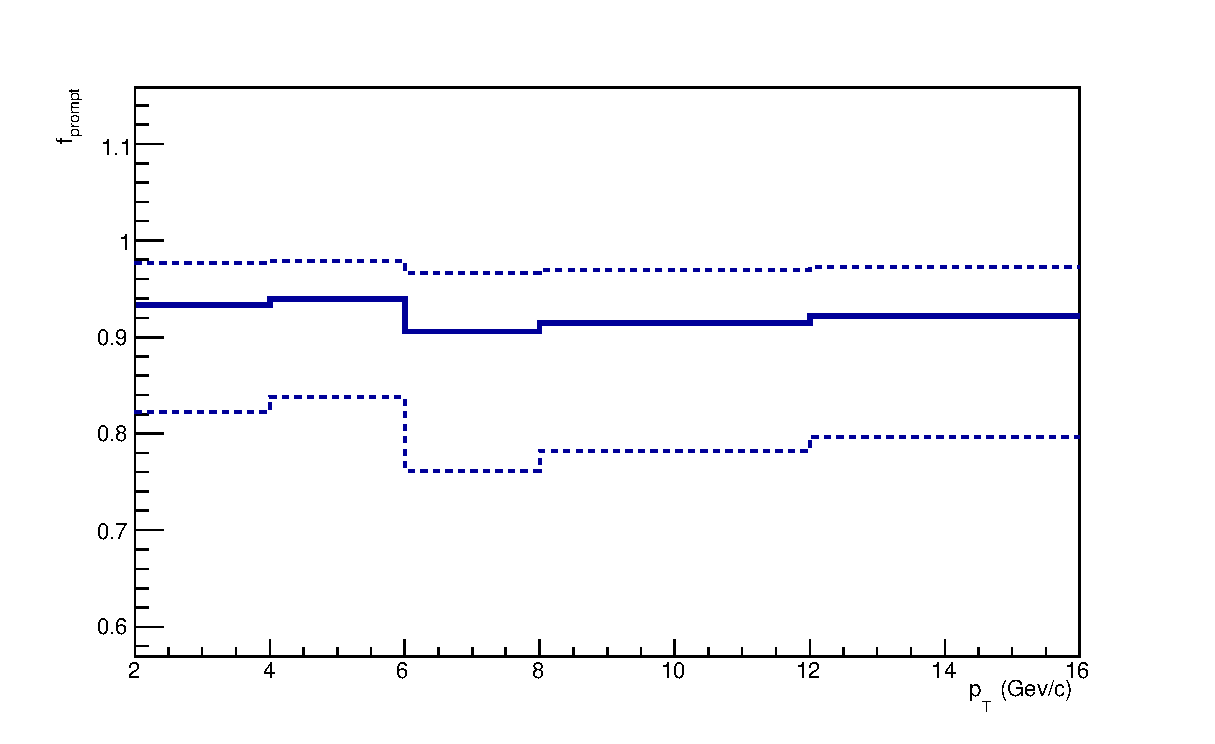
\includegraphics[width=7cm]{FigCap5/fprompt_3050.eps}
\caption{Values of fprompt for the $\Dplus$, $\Dzero$ and $\Ds$ mesons respectively.}
\label{fig:fPrompt}
\end{figure}

\section{Results}
\label{sec:PbPbResults}
The transverse-momentum distributions d$N$/d$\pt$ of prompt $\Ds$ meson 
is shown in Fig.~\ref{fig:DmesCorrYields010}
for the 0--10\%, 30--50\% and 60--80\% centrality classes. 
The vertical bars represent the statistical uncertainties, the empty boxes
the systematic uncertainties from the data analysis, and the shaded boxes
the systematic uncertainty due to the subtraction of the feed-down from 
B-hadron decays. The uncertainty on the branching ratios is quoted separately.
%Uncertainties on the pp cross section
%normalisation and on the branching ratios are quoted separately.

\begin{figure}[!t]
 \begin{center}
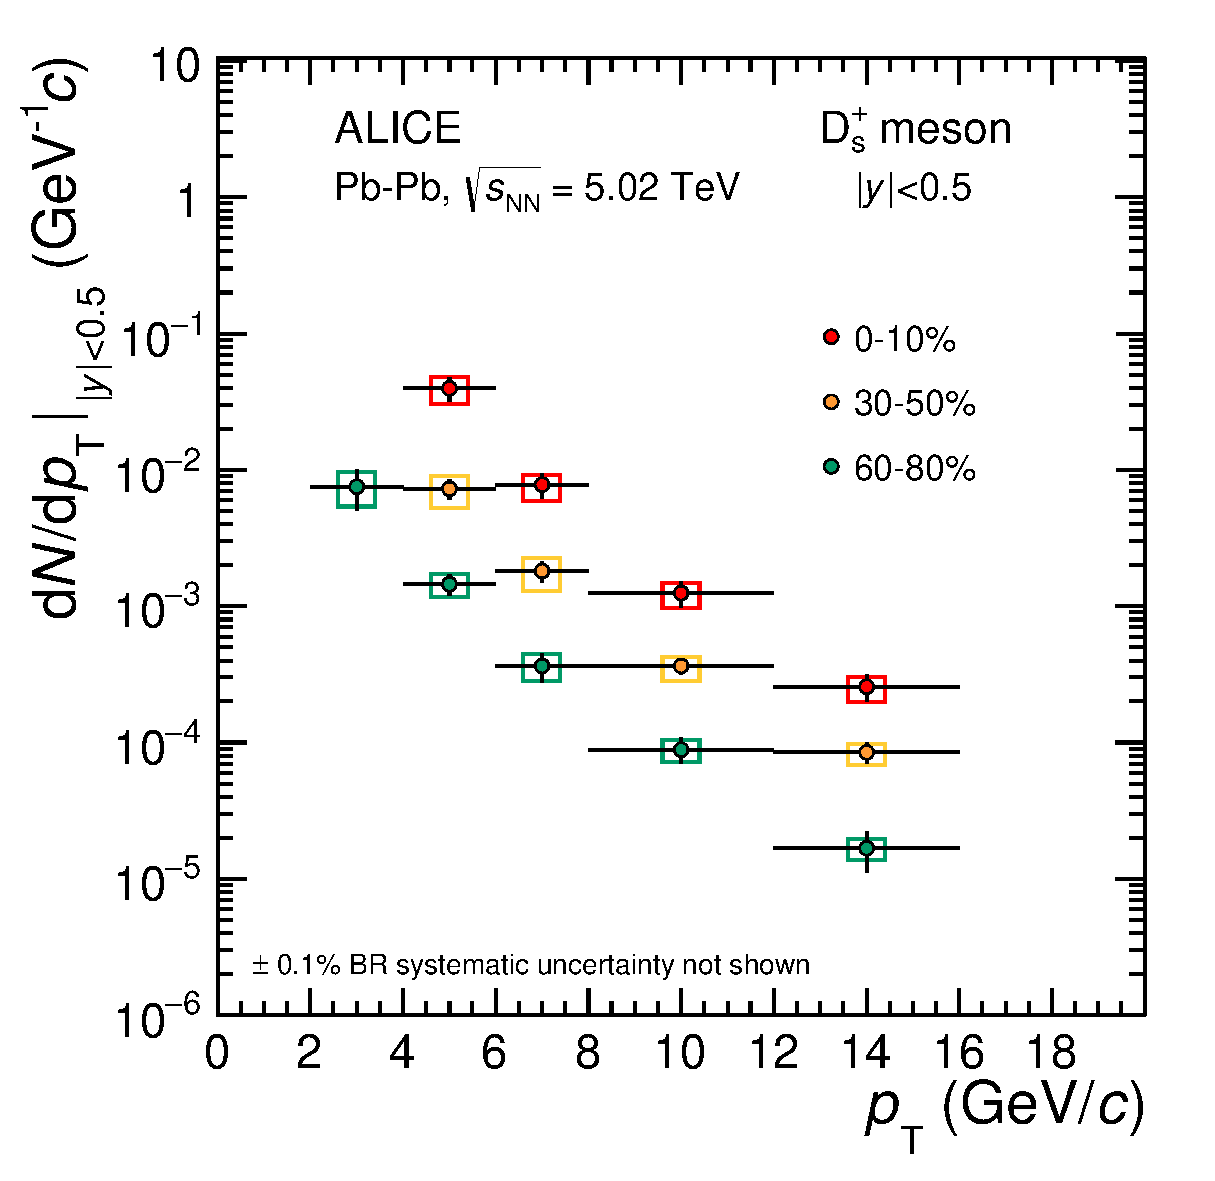
\includegraphics[angle=0, width=7.5cm]{FigCap5/Ds_dNdpt_010_3050_6080.eps}
 \end{center}
 \caption{Transverse momentum distributions d$N$/d$\pt$ of 
prompt $\Dzero$ (a), $\Dplus$ (b), $\Dstar$ (c) and $\Ds$ (d)  mesons in the 0--10\%, 30--50\% and 60--80\% 
centrality classes in $\PbPb$ collisions 
at $\sqrtsNN=5.02~\tev$. 
Statistical uncertainties (bars), systematic uncertainties from data 
analysis (empty boxes) and from feed-down subtraction 
(shaded boxes) are shown. 
Horizontal bars represent bin widths, symbols are placed at the centre of 
the bin. }
 \label{fig:DmesCorrYields010} 
\end{figure} 



Figure~\ref{fig:DmesRatio} shows the $\pt$-dependent ratios of
$\Dplus$/$\Dzero$, $\Dstar$/$\Dzero$, $\Ds/\Dzero$ and $\Ds/\Dplus$ meson yields, 
compared to the values measured in pp collisions at $\sqrt s=7~\tev$~\cite{Acharya:2017jgo}. 
%and central Pb--Pb collisions at $\sqrtsNN=2.76~\tev$~\cite{Adam:2015sza}. 
The $\Dplus$/$\Dzero$ and $\Dstar$/$\Dzero$ ratios are compatible in Pb--Pb and pp collisions, 
indicating no significant modification of their relative abundances. 
The $\Ds/\Dzero$ and $\Ds/\Dplus$ ratios are measured with better precision at 5.02~TeV with respect to 2.76~TeV.
The central values of these ratios are larger in Pb--Pb than in pp collisions, in all three centrality classes, however
the measurements in the two systems are compatible within about one standard deviation of the combined uncertainties.
\iffalse

\begin{figure}[!t]
\includegraphics[width=0.49\textwidth]{FigCap5/RatioDplusDzero-PbPb-010-3050-6080-502-pp-7.eps}
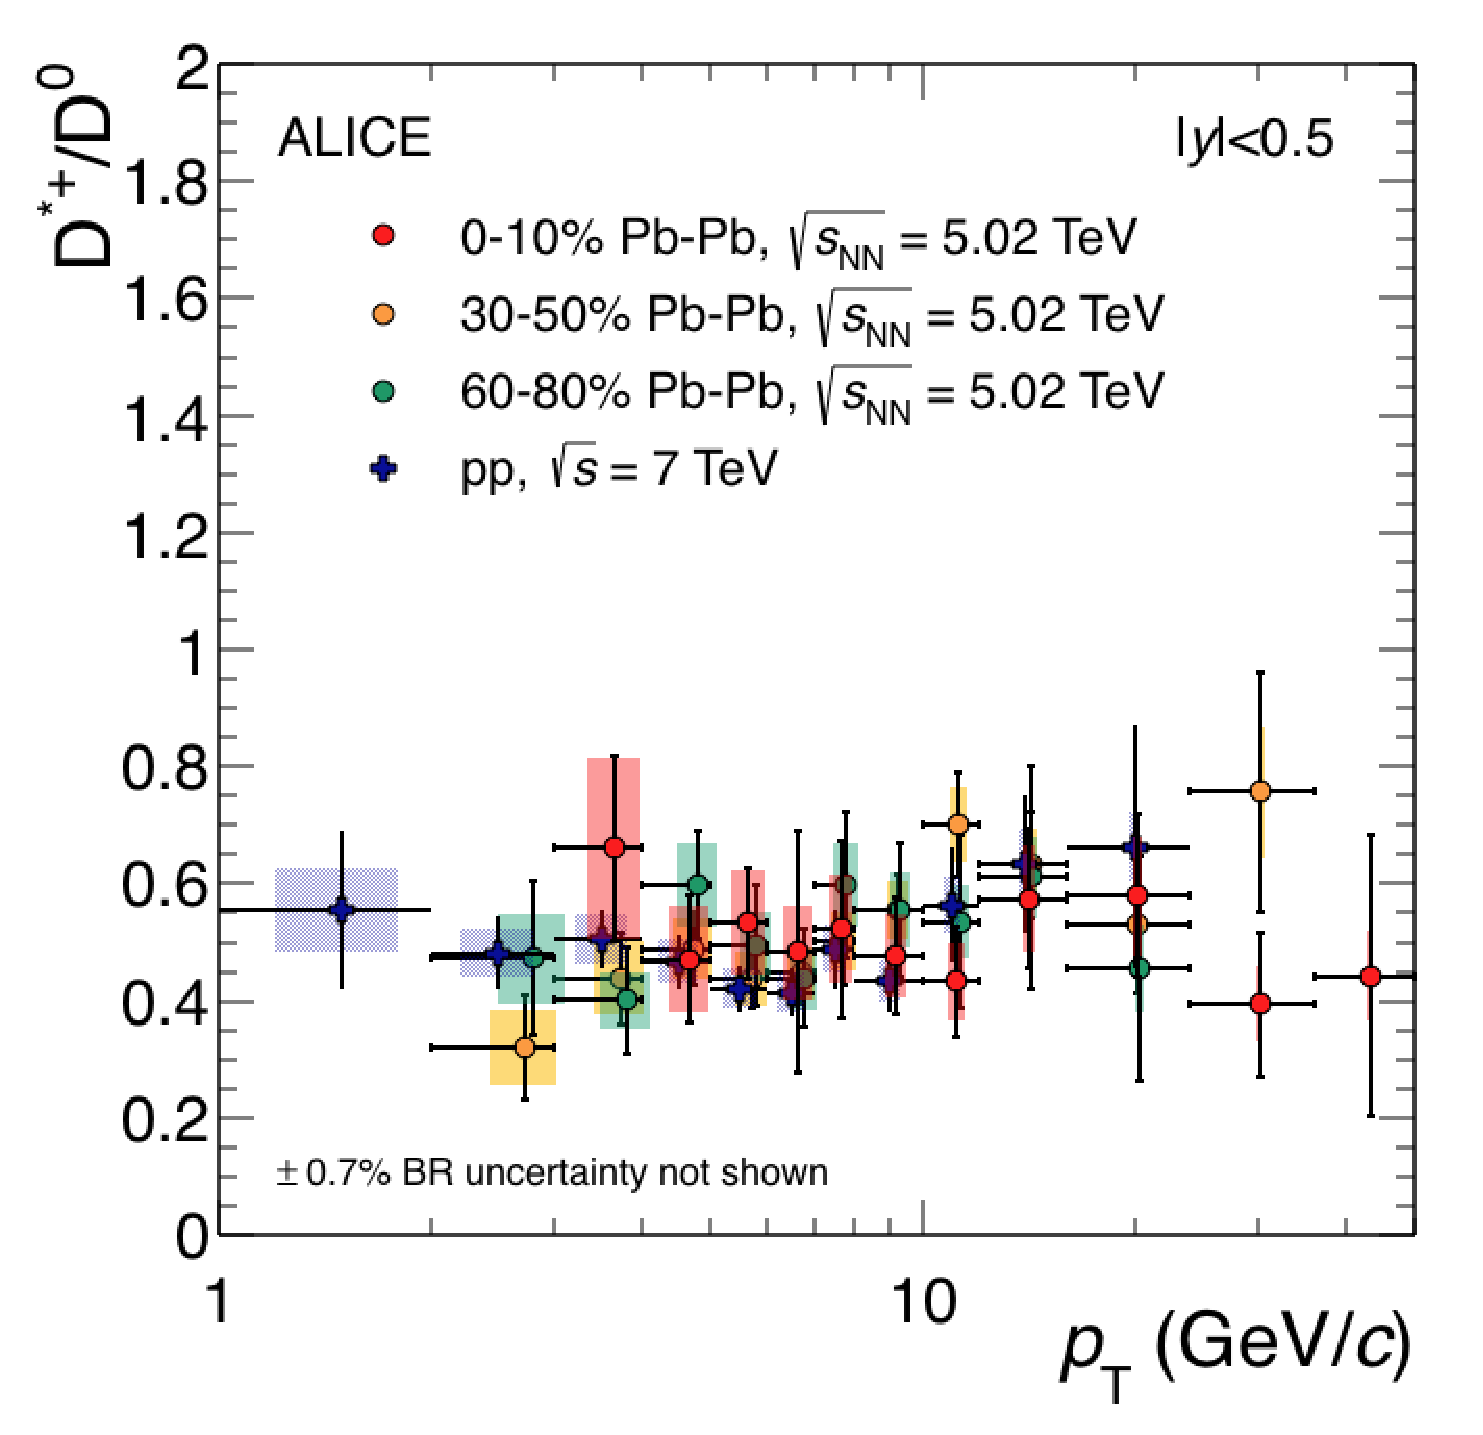
\includegraphics[width=0.49\textwidth]{FigCap5/RatioDstarDzero-PbPb-010-3050-6080-502-pp-7.eps}
 \label{fig:DmesRatio} 
\end{figure} 


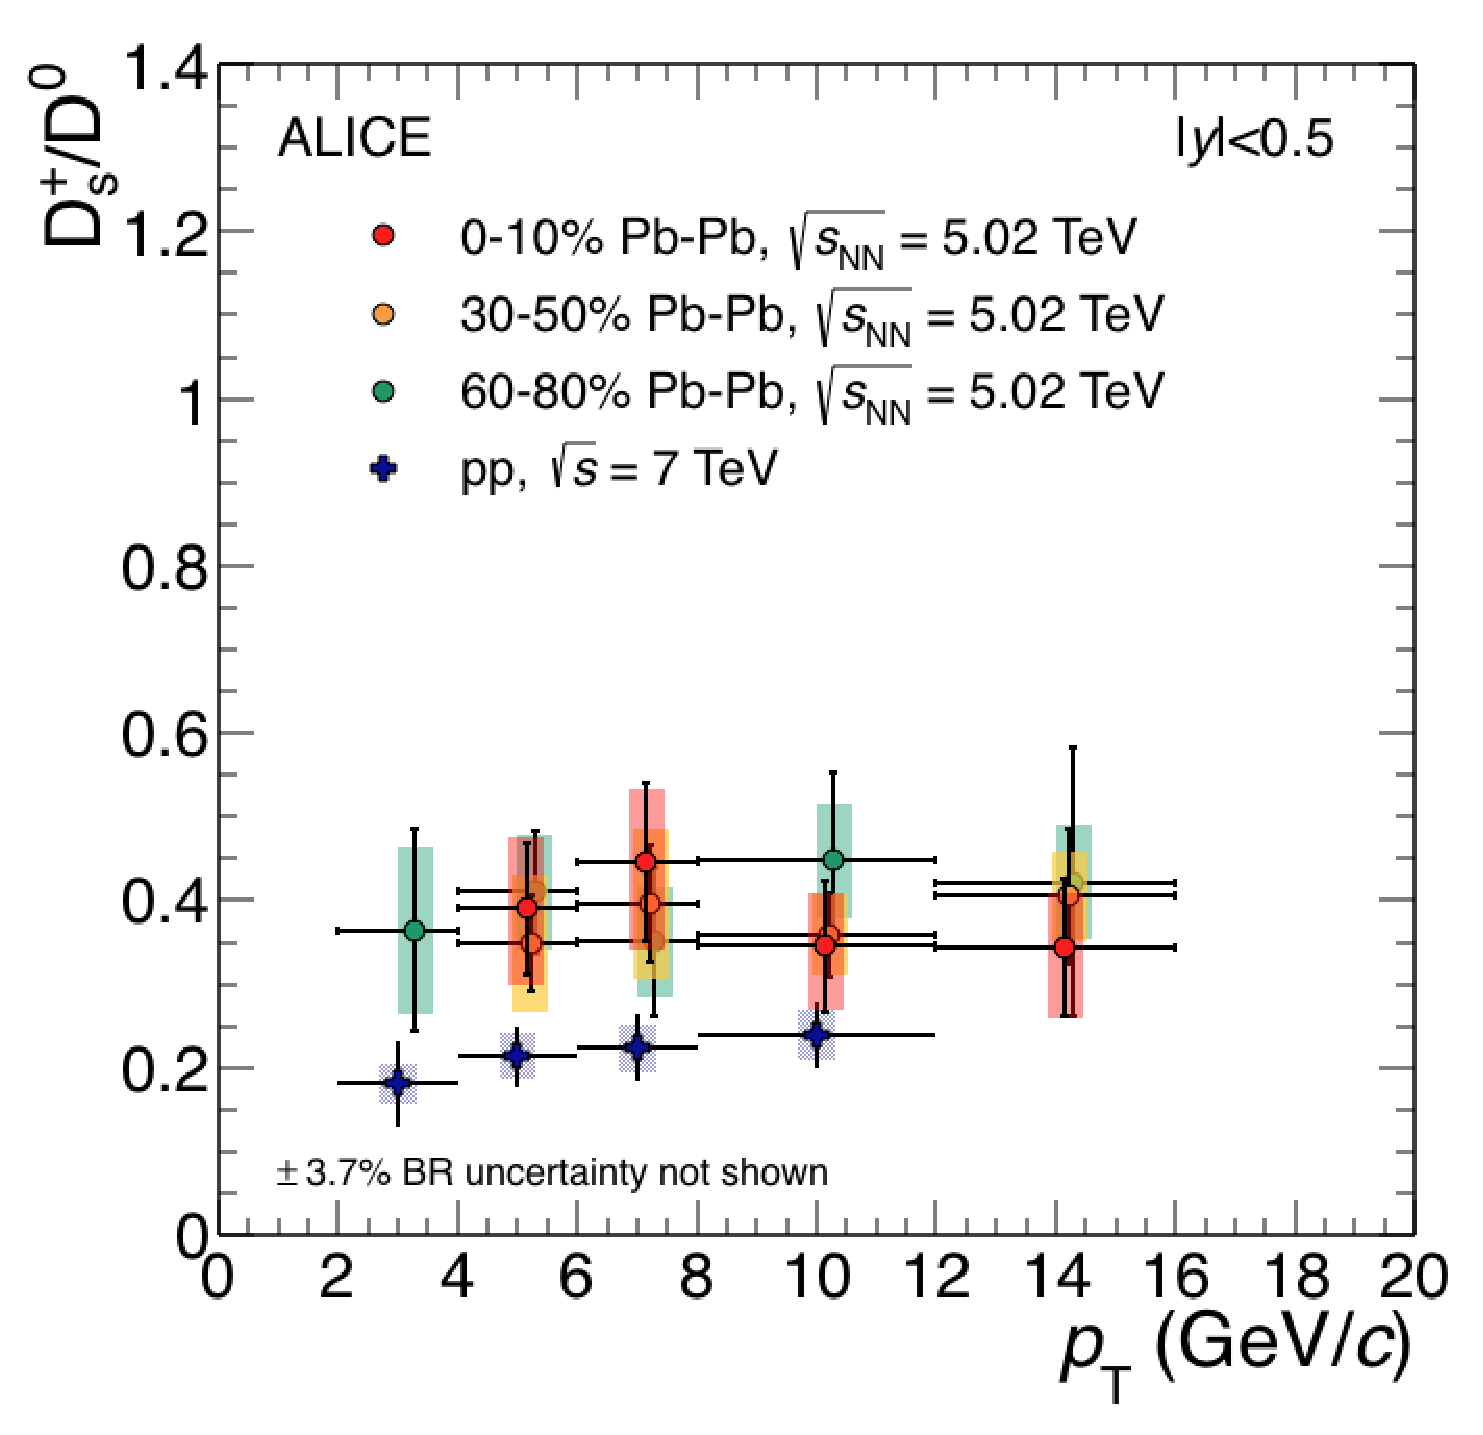
\includegraphics[width=0.49\textwidth]{FigCap5/RatioDsD0-PbPb-010-3050-6080-502-pp-7.eps}
\includegraphics[width=0.49\textwidth]{FigCap5/RatioDsDplus-PbPb-010-3050-6080-502-pp-7.eps}

\begin{figure}[!h]
\centering
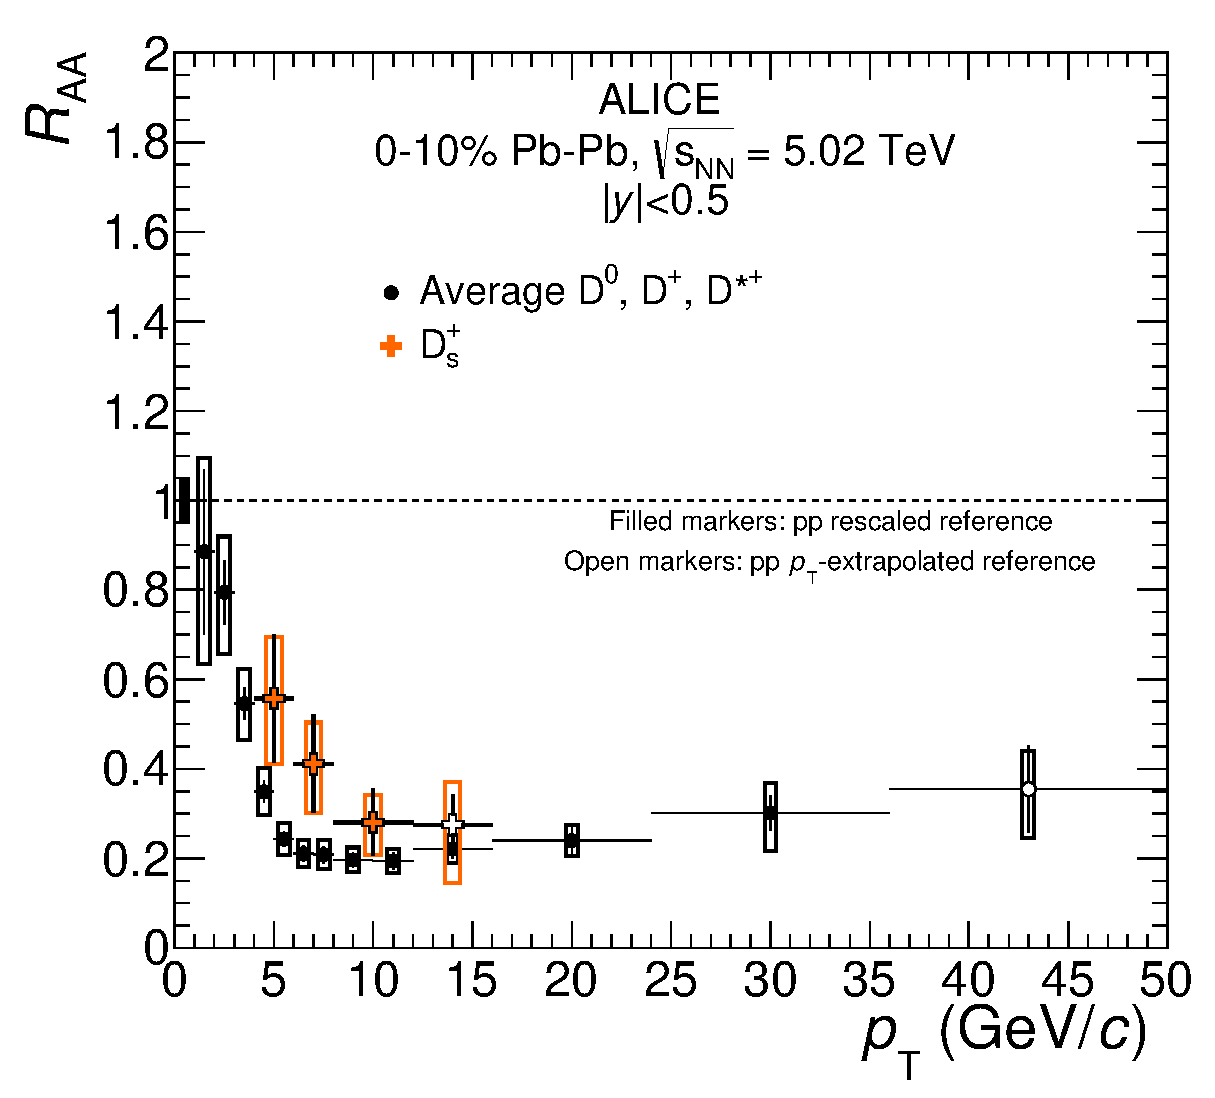
\includegraphics[angle=0, width=0.45\textwidth]{FigCap5/DmesonAverageDs_010_.eps}
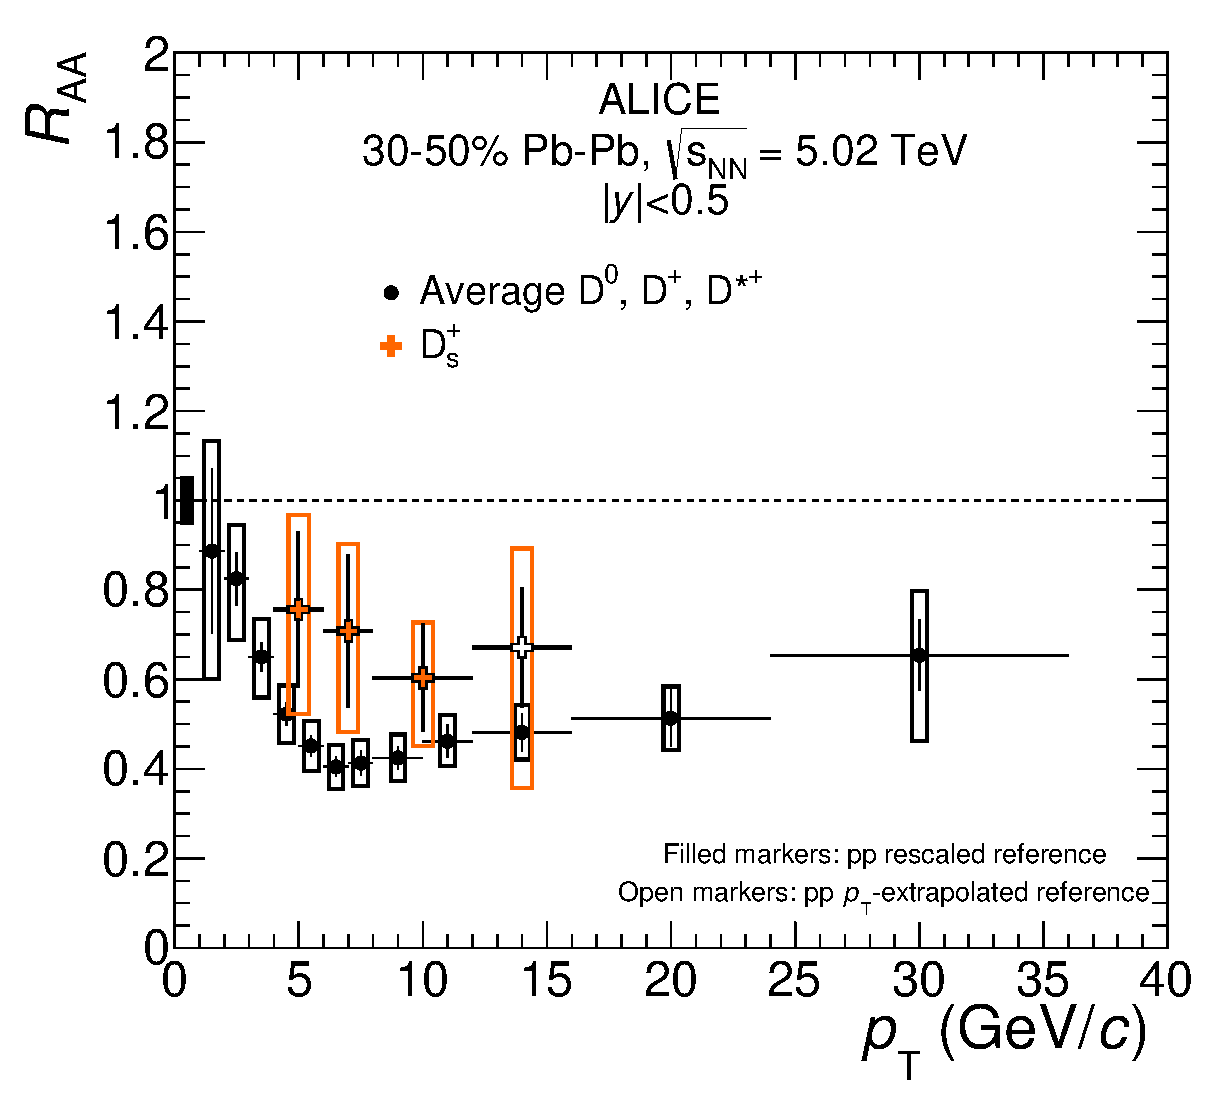
\includegraphics[angle=0, width=0.45\textwidth]{FigCap5/DmesonAverageDs_3050_.eps}
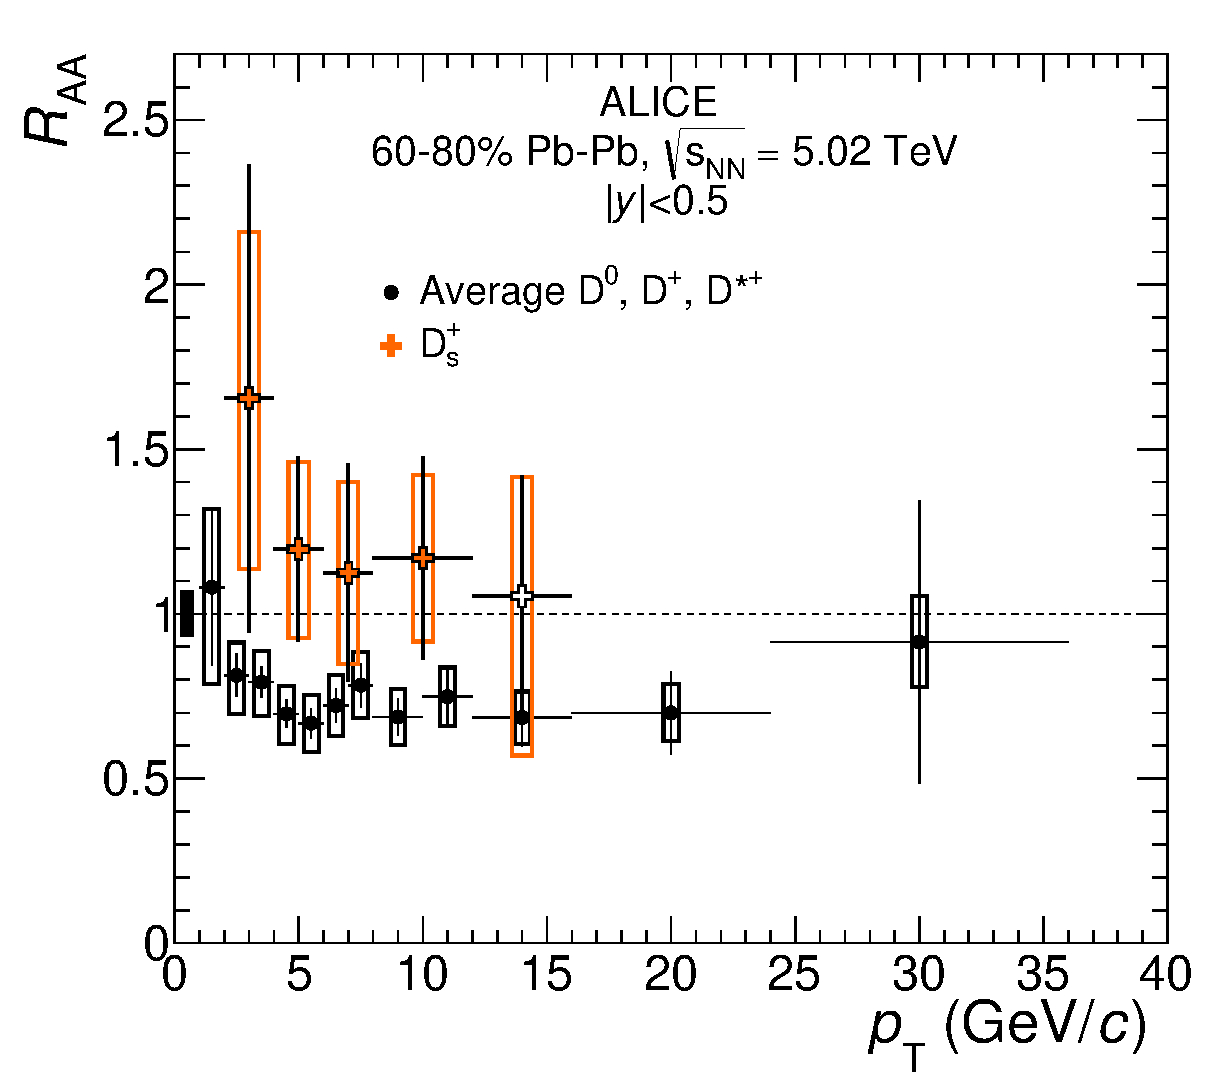
\includegraphics[angle=0, width=0.45\textwidth]{FigCap5/DmesonAverageDs_6080_.eps}
 \caption{$\RAA$ 
  of prompt $\Ds$ mesons 
  compared with the average $\RAA$ of$\Dzero$, $\Dplus$ and $\Dstar$ mesons for the 
0--10\%, 30--50\% and 60--80\%. 
Statistical (bars),  systematic (empty boxes), and normalisation (shaded box) 
uncertainties are shown.}
 \label{fig:DmesRaa} 
\end{figure} 

\fi

The average nuclear modification factors in the 0--10\% 
and 30--50\% centrality classes (right-hand panels of 
Fig.~\ref{DmesRaa}) show a suppression that is
maximal at $\pt=6$--$10~\gev/c$, where a reduction of the yields by
a factor of about 5 and 2.5 with respect to the binary-scaled
 pp reference is observed in the two centrality classes, respectively.
The suppression decreases with decreasing $\pt$ for $\pt<6~\GeV/c$, and 
$\RAA$ is compatible with unity  in the interval $1<\pt<3~\gev/c$.
The average $\RAA$ in the 60--80\% centrality class shows a 
suppression by about 20--30\%, without a pronounced dependence on $\pt$.

The $\Raa$ of prompt $\Ds$ mesons is shown in the 
right-hand panels of Fig.~\ref{DmesRaa},
where it is compared with the average $\Raa$ of non-strange 
D mesons: the central values are
larger for $\Ds$ mesons, but the two measurements are 
compatible within one standard deviation of the combined 
uncertainties, as in the case of the ratios shown in Fig.~\ref{DmesRatio}.



Models based on heavy-quark transport and models based
 on perturbative QCD calculations of parton energy loss 
 are shown on the left and on the right, respectively.
Transport models in the left panels include: 
POWLANG~\cite{Beraudo:2014boa} and TAMU~\cite{He:2014cla}, 
in which the interactions are only described by collisional (i.e.\,elastic) processes; 
BAMPS-el+rad~\cite{Uphoff:2014hza}, LBT~\cite{Cao:2017hhk} 
and PHSD~\cite{Song:2015ykw}, in which also energy loss 
from medium-induced gluon radiation
is considered, in addition to collisional process.
In the right panels, the CUJET3.0~\cite{Xu:2015bbz}, 
Djordjevic~\cite{Djordjevic:2015hra} and MC@sHQ+EPOS2~\cite{Nahrgang:2013xaa}
 models include both radiative and collisional energy loss processes, and
the SCET~\cite{Kang:2016ofv} model includes 
medium-induced gluon radiation and a mechanism of formation
 and dissociation of heavy-flavour hadrons in the QGP.
All models, with the exception of BAMPS and CUJET3.0, include 
a nuclear modification of the parton distribution functions.
The LBT, MC@sHQ, PHSD, POWLANG and TAMU
models include a contribution of hadronisation via quark 
recombination, in addition to independent fragmentation. 
Most of the models provide a fair description of the data in the
 region $\pt<10~\gev/c$ in central collisions, 
but many of them (LBT, PHSD, POWLANG and SCET) provide 
a worse description of non-central collisions.
In the high-$\pt$ region above $10~\gev/c$ only the BAMPS, 
CUJET3.0, Djordjevic and SCET models can describe the data. 
The CUJET3.0 and Djordjevic models provide a 
fair description of the $\RAA$ in all three centrality classes for 
$\pt > 5-10~\gev/c$, where radiative energy loss is expected to 
be the dominant interaction mechanism, suggesting that the 
dependence of radiative energy loss on the path length of 
charm quarks in the hot and dense medium is well understood. 

In Fig.~\ref{DandDsRaaWithModels},  the non-strange and 
strange D-meson $\RAA$ are compared with  
the models that provide both observables. A large increase of
 the $\Ds$ $\RAA$ is expected in the two models, PHSD and 
 TAMU, in particular for $\pt<5~\gev/c$, with respect to 
 non-strange D mesons. This increase is induced by hadronisation 
 via quark recombination in a strangeness-rich QGP, as well as by different 
interaction cross sections for non-strange D and for $\Ds$ in 
the hadronic phase of the system evolution. It is interesting
 to note that the TAMU model gives a larger effect than the 
 PHSD model and that the central values of the two measured $\RAA$ differ also 
in the region around $\pt=10~\gev/c$, where the effect in the 
models becomes small, although the present experimental 
uncertainties prevent us from drawing a firm conclusion. 

The simultaneous comparison of $\RAA$ and elliptic flow 
$v_2$ measurements at $\sqrtsNN=5.02~\tev$~\cite{Acharya:2017qps} 
with models can provide more stringent constraints to the 
implementation of the interaction and hadronisation processes for heavy quarks. 
This comparison is shown in Fig.~\ref{RAAandv2} for the $\RAA$  
and $v_2$, in the 0--10\% and 30--50\% centrality classes
 respectively, together with models that provide 
 simultaneous description of the observables.
The level of model-to-data consistency was quantified in
 terms of the reduced $\chi^2$ in the respective $\pt$ interval 
 where the calculations are available.
Values of reduced $\chi^2$ for $\RAA$ measurements in 
0--10\% and 30--50\% centrality classes and $v_2$ in 30--50\% 
centrality class are reported in Table~\ref{tab:RedChi2}.
TAMU model overestimates $\RAA$ at high $\pt$ in central 
events and describes the magnitude of the elliptic flow, 
but fails in reproducing the shape.
BAMPS-el overestimates the maximum flow while 
underestimating the suppression at high $\pt$. The 
radiative term in BAMPS-el+rad improves the description 
of the $\RAA$ but gives a smaller than observed maximum
 $v_2$.~PHSD, POWLANG, LBT and MC@sHQ provide
  instead a fair description of both $v_2$ magnitude and shape
as well as of energy loss, as their values of $\chi^2/$ndf indeed show. 
	\iffalse

\begin{figure}[!t]
 \begin{center}
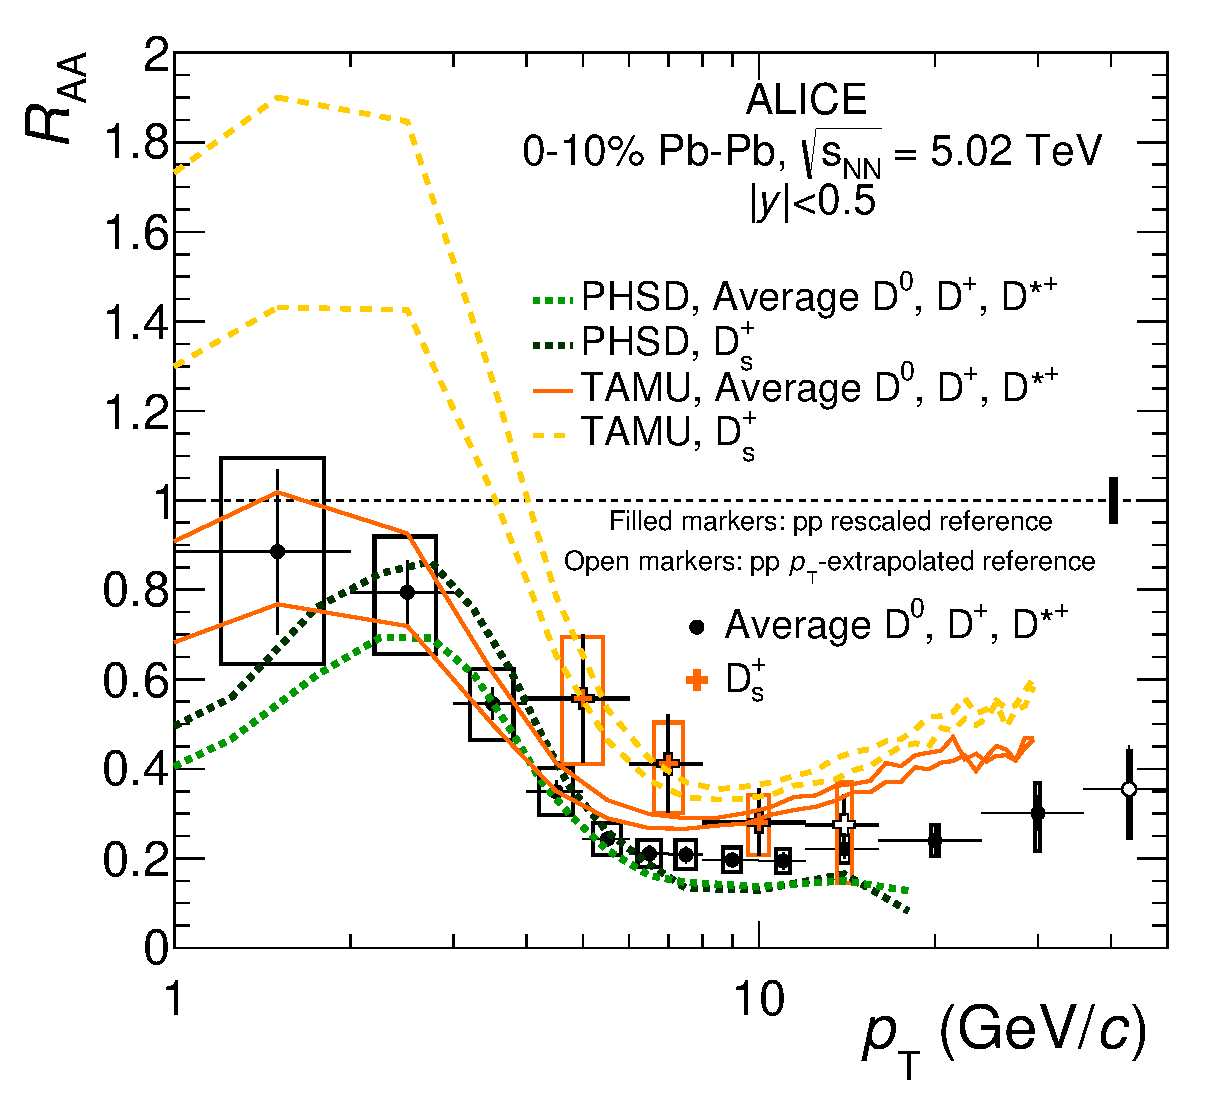
\includegraphics[angle=0, width=0.49\textwidth]{FigCap5/DmesonAverageDs_010_Models_logx_.eps}
 \end{center}
 \caption{Average $\RAA$ of $\Dzero$, $\Dplus$ and $\Dstar$ mesons and $\RAA$ of $\Ds$ mesons in the 0--10\% centrality class compared with the PHSD~\cite{Song:2015ykw}  and TAMU~\cite{He:2014cla} model calculations.}
 \label{DandDsRaaWithModels} 
\end{figure} 

\begin{figure*}[!t]
\begin{center}
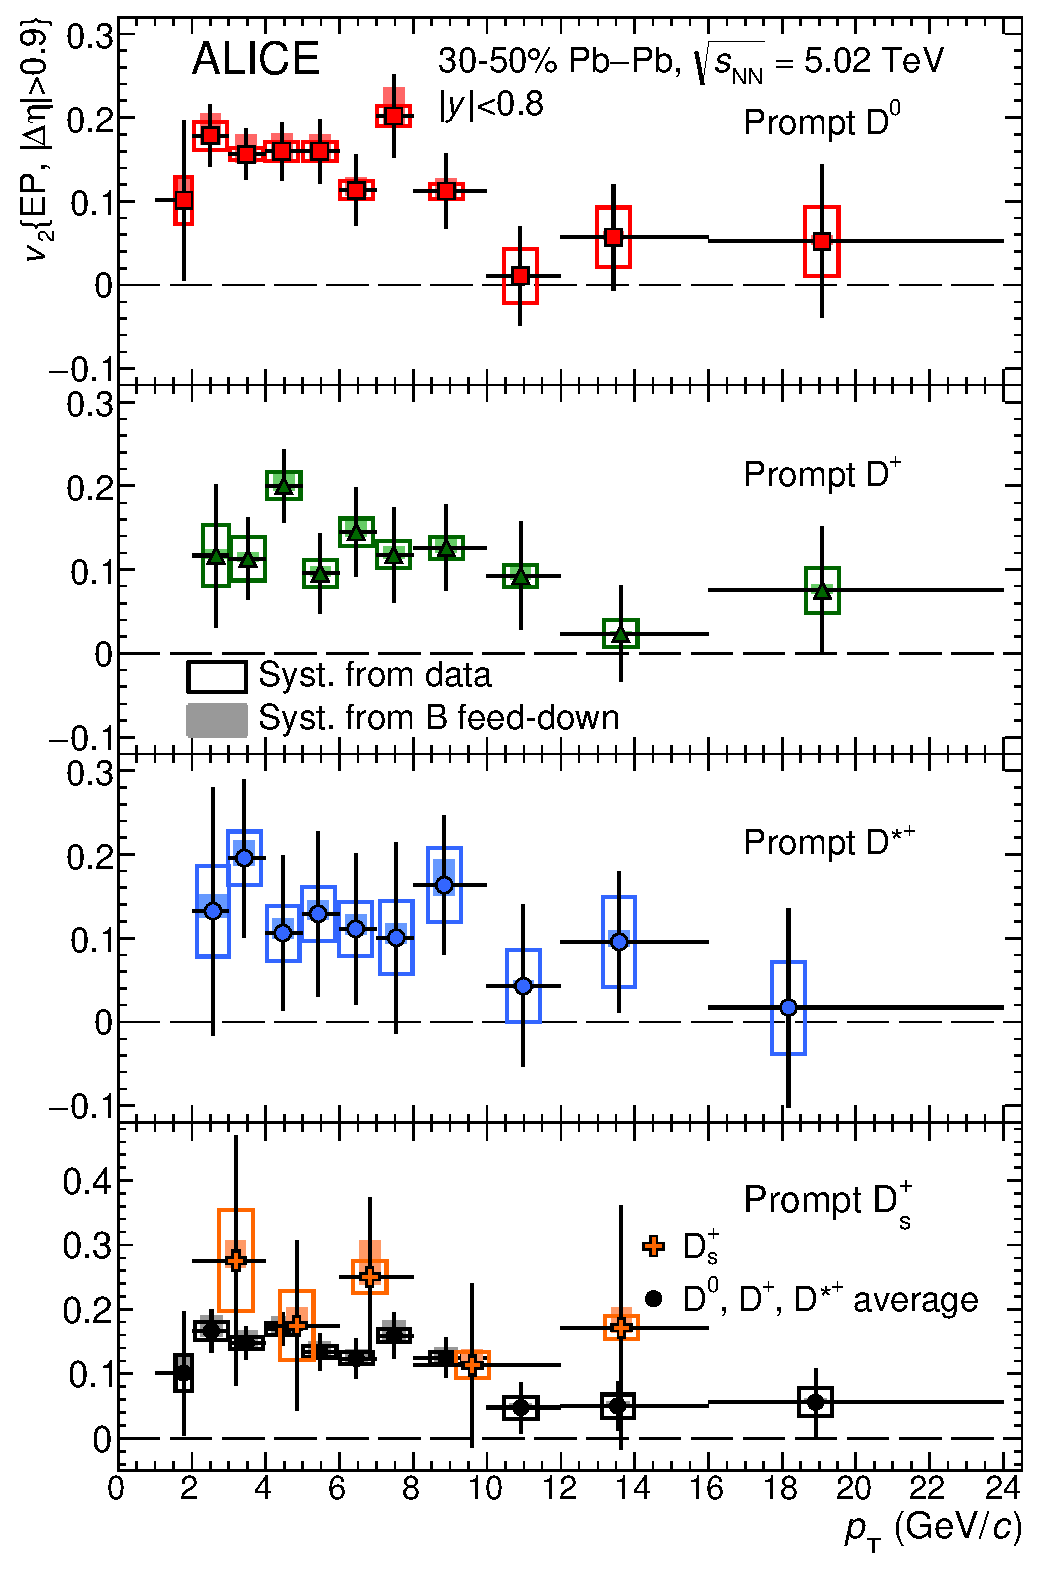
\includegraphics[width=.65\textwidth]{FigCap5/4mesons4pads.eps}
\caption{Elliptic flow $v_2$ as a function of $\pt$ for prompt $\Dzero$, $\Dplus$, 
$\Dstar$ and $\Ds$ mesons and their charge conjugates for 
$\PbPb$ collisions in the centrality class 30--50\%.
The bottom panel also shows the average
$v_2$ of $\Dzero$, $\Dplus$ and $\Dstar$. The symbols are positioned
horizontally at the average $\pt$ of the reconstructed D mesons. %four D-meson species.
%The central value was obtained with the assumption 
%$v_2^{\rm feed\mbox{-}down}=v_2^{\rm prompt}$.
%The minimum separation in pseudorapidity between D mesons and the particles used to determine $\psi_2$ is indicated ($|\Delta\eta|>0.9$).
Vertical error bars represent the statistical uncertainty, empty boxes the systematic 
uncertainty associated with the D-meson anisotropy measurement and the event-plane 
resolution. Shaded boxes show the feed-down uncertainty.}
\label{fig:v2_4mesons} 
\end{center}
\end{figure*}

\fi
The $v_2$ of prompt $\Dzero$, $\Dplus$, $\Dstar$ and $\Ds$ mesons in
the 30--50\% centrality class is shown as a function of $\pt$ in Fig.~\ref{fig:v2_4mesons}.
%{\bf The meaning of the error bars is described in the figure caption, I would not repeat here.}
The symbols are positioned at the average $\pt$ of the 
reconstructed D mesons: this value was determined as the 
average of the $\pt$ distribution of candidates in the signal invariant-mass region, 
after subtracting the contribution of the background 
candidates estimated from the side bands.
The $v_2$ of $\Dzero$, $\Dplus$ and $\Dstar$ are consistent 
with each other and they are larger than zero in $2<\pt<10~\gev/c$.
The average of the $v_2$ measurements for $\Ds$ mesons in
 the three $\pt$ intervals within $2<\pt<8~\gev/c$ is 
 positive with a significance of 2.6\,$\sigma$,
where $\sigma$ is the uncertainty of the average $v_2$, 
calculated using quadratic error propagation for the
 statistical and uncorrelated systematic uncertainties 
(signal extraction) and linear propagation for the correlated 
systematic uncertainties ($R_2$ and feed-down correction).
The average $v_2$ and $\pt$ of $\Dzero$, $\Dplus$ and 
$\Dstar$, shown in the bottom panel of Fig.~\ref{fig:v2_4mesons}, was 
computed using the inverse of the squared statistical uncertainties as weights. 
The systematic uncertainties were propagated by
treating the contributions from $R_2$
and the feed-down correction as correlated among D-meson species. 
